% ============================================================
%  analisis_resultados.tex
%  Analysis of the figures of the sedimentary segregation model
%  in bidisperse hydraulic dunes
% ============================================================
\documentclass[12pt, a4paper]{article}

% --- Packages ---
\usepackage[T1]{fontenc}
\usepackage[utf8]{inputenc}
\usepackage[english]{babel}
\usepackage{lmodern}
\usepackage{geometry}
\geometry{margin=2.5cm}

\usepackage{graphicx}
\usepackage{subcaption}
\usepackage{float}
\usepackage{amsmath, amssymb}
\usepackage{booktabs}
\usepackage{xcolor}
\usepackage{hyperref}
\hypersetup{
    colorlinks = true,
    linkcolor  = blue!60!black,
    citecolor  = blue!60!black,
    urlcolor   = blue!60!black,
}

% Relative path to figures
\graphicspath{{figures/}}

% ============================================================
\title{%
    \textbf{Results Analysis}\\[0.4em]
    \large Influence of Sedimentary Segregation on the Dynamics
    of Hydraulic Dunes: Bidisperse Model}
\author{Felipe Espinoza}
\date{\today}
% ============================================================

\begin{document}
\maketitle
\tableofcontents
\newpage

% ============================================================
\section{Introduction and Model Context}
% ============================================================

This document analyzes the figures generated by the numerical model of
sedimentary segregation in bidisperse hydraulic dunes. The system
studies how mixtures of two grain sizes ---fines ($d_s = 0.30$\,mm)
and coarse ($d_l = 1.00$\,mm)--- reorganize vertically while the
dune migrates under an oscillatory hydraulic flow.

The narrative is organized to build physical understanding progressively:
we begin with the global space--time picture of the segregation process
(Sec.~\ref{sec:fan}), then zoom into the time-averaged vertical structure
(Sec.~\ref{sec:sorting}), reveal the flow mechanism responsible for
trapping coarse grains (Sec.~\ref{sec:velocity}), isolate the role of
granular diffusion (Sec.~\ref{sec:diffusion}), examine the time evolution
of the profile (Sec.~\ref{sec:temporal}), and finally quantify the
length-scales that govern the segregation--diffusion competition
(Sec.~\ref{sec:peclet}).
Temporal convergence of the simulations is documented in
Appendix~\ref{app:convergence}.

\subsection*{Fundamental variables and conventions}

\begin{itemize}
    \item $\phi_s$ is the \textbf{volumetric fraction of fines}: $\phi_s = 1$
          corresponds to pure fine sediment and $\phi_s = 0$ to pure coarse.
    \item $\eta = z/h$ is the \textbf{normalized vertical coordinate}: $\eta = 0$
          is the impermeable base and $\eta = 1$ the free surface. The local
          bed thickness varies between $h = 1.00$\,mm (flat bed) and
          $h = 9.00$\,mm (crest).
    \item $\langle \phi_s \rangle_x(\eta)$ is the \textbf{average in $x$} over
          the dune body, weighted by $h(x)$ (volume average).
    \item $\eta_a$ is the \textbf{roof of the buried deposit}: below
          this height the material has already left the active layer ($\delta_a = 1.5$\,mm)
          and its composition is frozen ($\langle\eta_a\rangle \approx 0.71$).
    \item $\ell$ is the \textbf{segregation--diffusion equilibrium length}:
          \begin{equation}
              \ell = \frac{D_{sl}}{f_{sl}} = \frac{A\,(C\bar{d} + p)}{B\,F(R,\phi_s)}
              \label{eq:ell}
          \end{equation}
          where $\dot{\gamma}$ cancels between $f_{sl}$ and $D_{sl}$, so
          $\ell$ does not depend on the hydraulic slope $i$.
    \item The \textbf{local Péclet number} $Pe = L/\ell$ measures how many interface
          thicknesses fit in the reference scale $L$:
          \begin{itemize}
              \item $L = h$: scale of the entire column.
              \item $L = \delta_a$: scale of the active layer (physically
                    relevant scale for burial).
          \end{itemize}
\end{itemize}

The main runs compare two physical configurations:
\begin{enumerate}
    \item \textbf{With granular diffusion} ($A = 0.108$, Trewhela et al.\ 2021):
          the diffusive term $D_{sl}$ broadens the compositional interfaces.
    \item \textbf{Without diffusion} (pure hyperbolic model, $D_{sl} = 0$): upper
          bound of the compositional contrast; the interfaces only broaden
          due to numerical dissipation.
\end{enumerate}

All runs in the main section were carried out until $t = 2400$\,s,
with mesh $N_x = 400$, $N_z = 40$, $U_0 = 3 \times 10^{-4}$\,m/s,
initial concentration $\phi_s^0 = 0.70$ unless otherwise indicated.

\newpage
% ============================================================
\section{Compositional Fan: Space--Time Overview of Segregation}
\label{sec:fan}
% ============================================================

The compositional fan is the starting point of the analysis because it provides
the most complete picture of the system: the entire temporal history of
$\phi_s(x,\eta)$ is visible at once, revealing \emph{how quickly} and
\emph{where} segregation reorganizes the sediment mixture.

\begin{figure}[H]
    \centering
    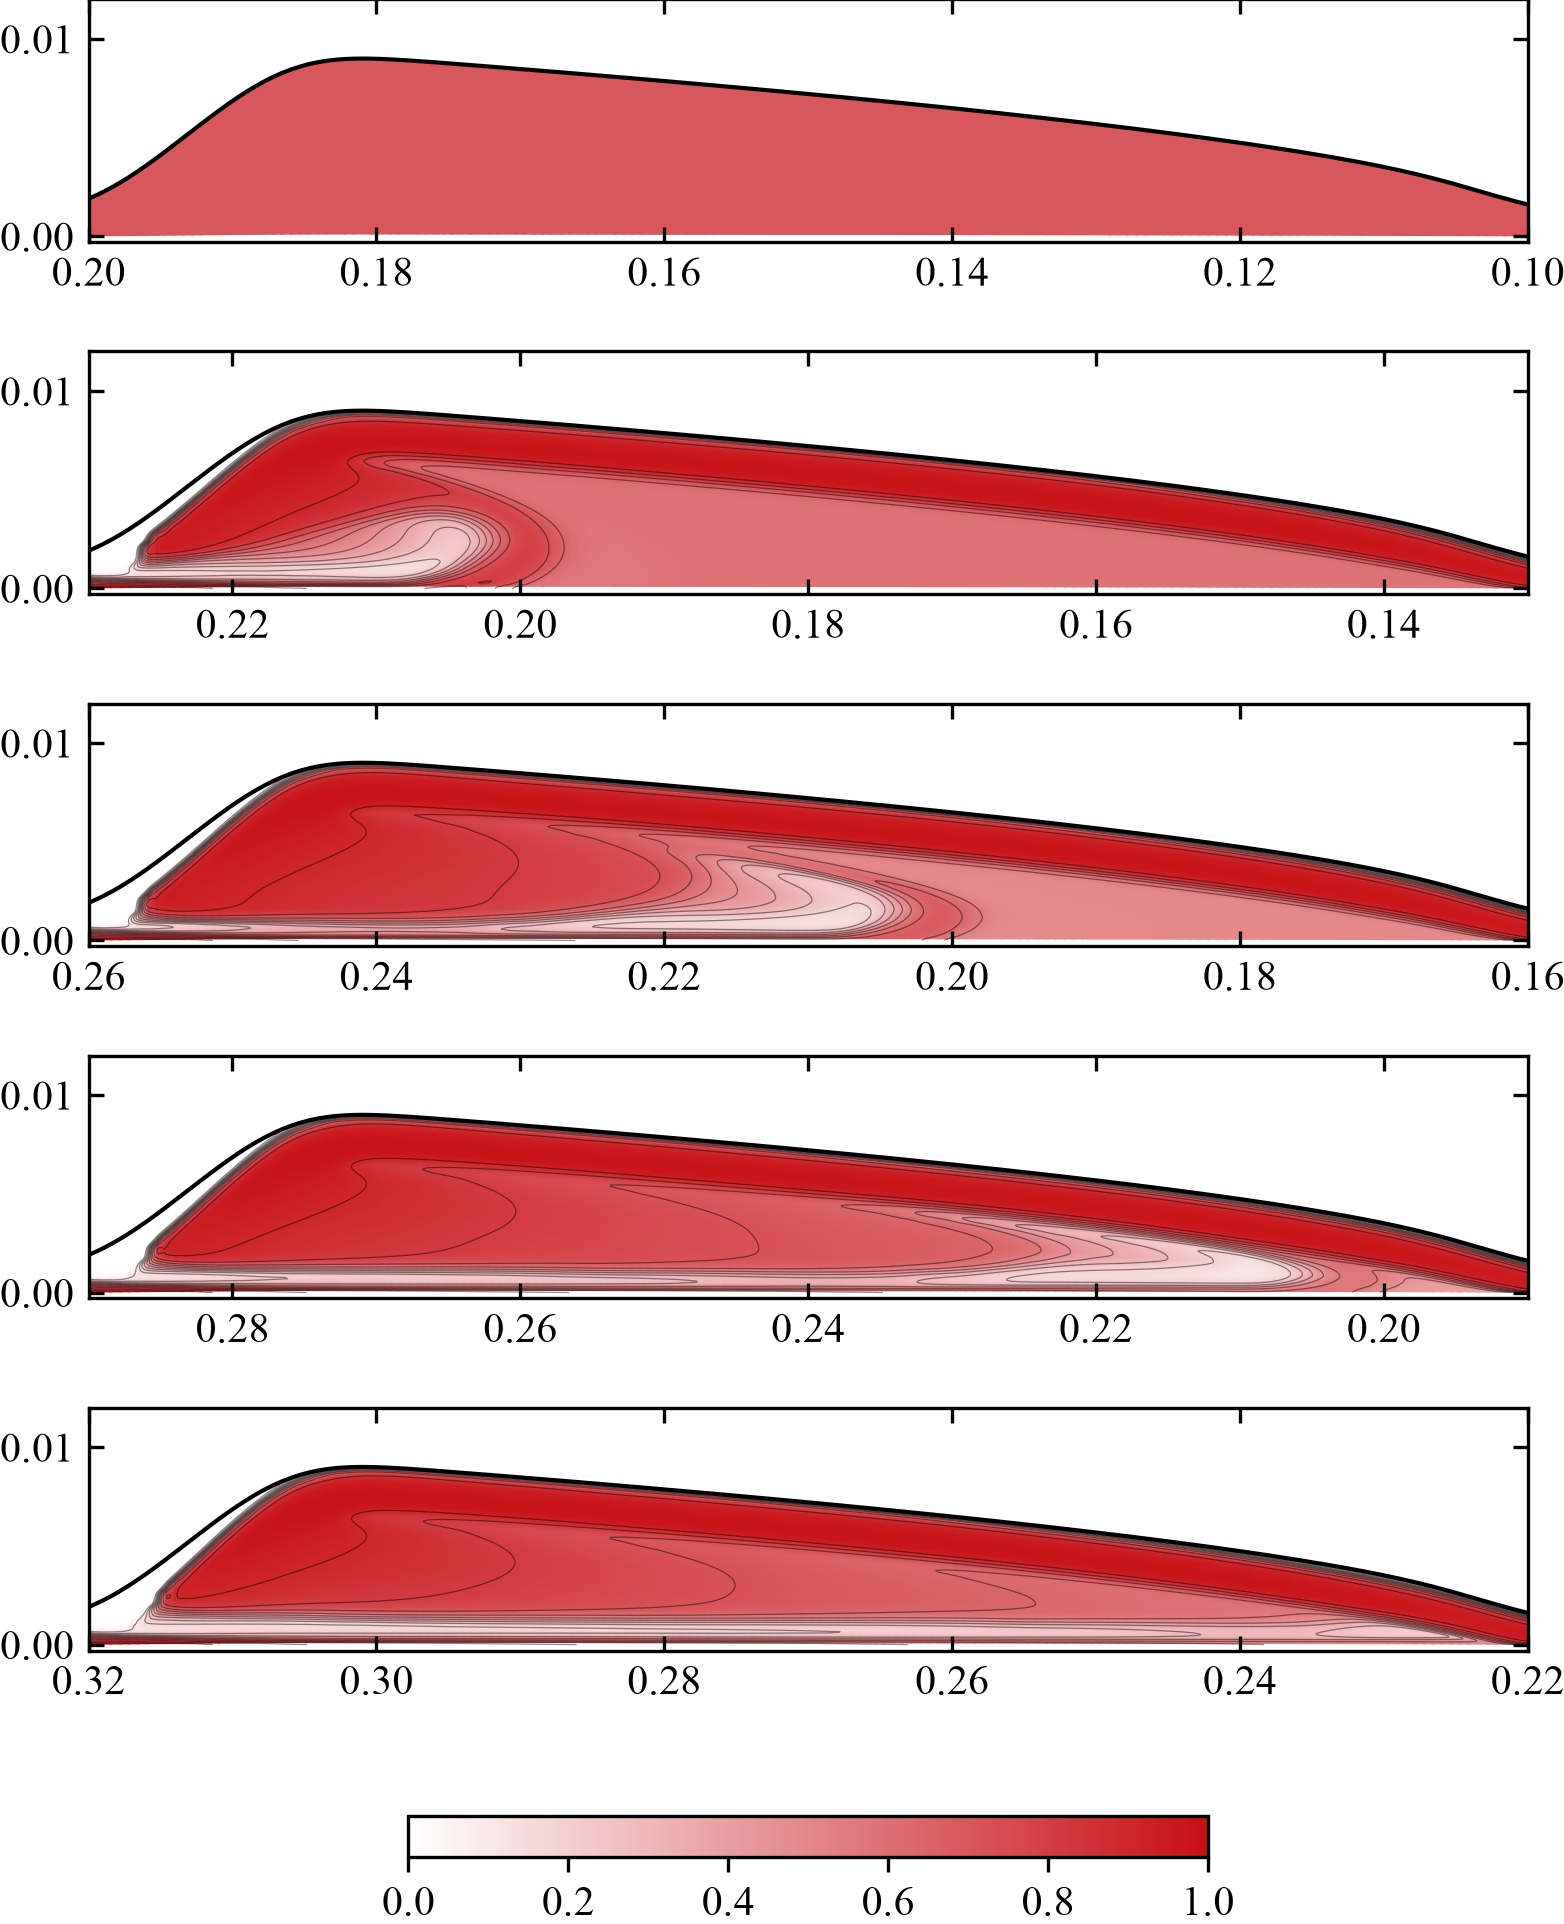
\includegraphics[width=\textwidth]{Slope_comparation_fan_i1_phi070.png}
    \caption{%
        \textbf{Compositional fan plot} for the run
        \textit{Slope comparation}, $\phi_s^0 = 0.70$, slope
        $i_1 = 0.00975$, $t = 2400$\,s.
        Each ``leaf'' of the fan corresponds to a temporal snapshot of
        $\phi_s(x,\eta)$ in the $\sigma$-mesh (normalized vertical coordinate
        vs.\ horizontal position), superimposed to visualize the temporal
        evolution of the segregation pattern from the uniform initial
        condition (innermost leaf) to the final state (outermost leaf).
    }
    \label{fig:fan}
\end{figure}

\subsection*{Analysis and interpretation}

The fan plot allows visualizing the complete temporal history of
segregation over the full dune geometry. Three key features emerge:

\begin{itemize}
    \item \textbf{Sorting front propagation velocity}: the angular separation
          between consecutive leaves quantifies how rapidly the system departs
          from the uniform initial state. The front advances quickly at first and
          progressively slows down, indicating that the system approaches
          (without reaching) a quasi-steady pattern within the simulated time.
    \item \textbf{Spatial modulation by dune geometry}: the effective front
          thickness varies with $x$, reflecting the locally variable bed height
          $h(x)$. Near the crest (thicker bed), the segregation front has more
          column to traverse and reaches a more developed state; near the
          stoss toe (thinner bed), the process is less complete.
    \item \textbf{Approach to a traveling wave}: if the late leaves collapse
          onto each other, the system tends toward a traveling-wave solution
          in the co-moving frame. The analysis shows that the system still moves
          by $\sim 11.5\%$ of the total change between $t = 2400$ and $4800$\,s
          (see Appendix~\ref{app:convergence}), confirming that the final
          snapshot is representative but not fully stationary.
\end{itemize}

The fan thus motivates the subsequent sections: it shows that segregation
builds a persistent large-scale pattern, whose vertical structure is
characterized in Section~\ref{sec:sorting} and whose physical mechanism is
identified in Section~\ref{sec:velocity}.

\newpage
% ============================================================
\section{Averaged Vertical Sorting Profile}
\label{sec:sorting}
% ============================================================

While the fan reveals the space--time evolution, the averaged vertical
profile $\langle\phi_s\rangle_x(\eta)$ condenses the outcome into a single
diagnostic that characterizes the final compositional state of the deposit.

\begin{figure}[H]
    \centering
    \begin{subfigure}[t]{0.32\textwidth}
        \centering
        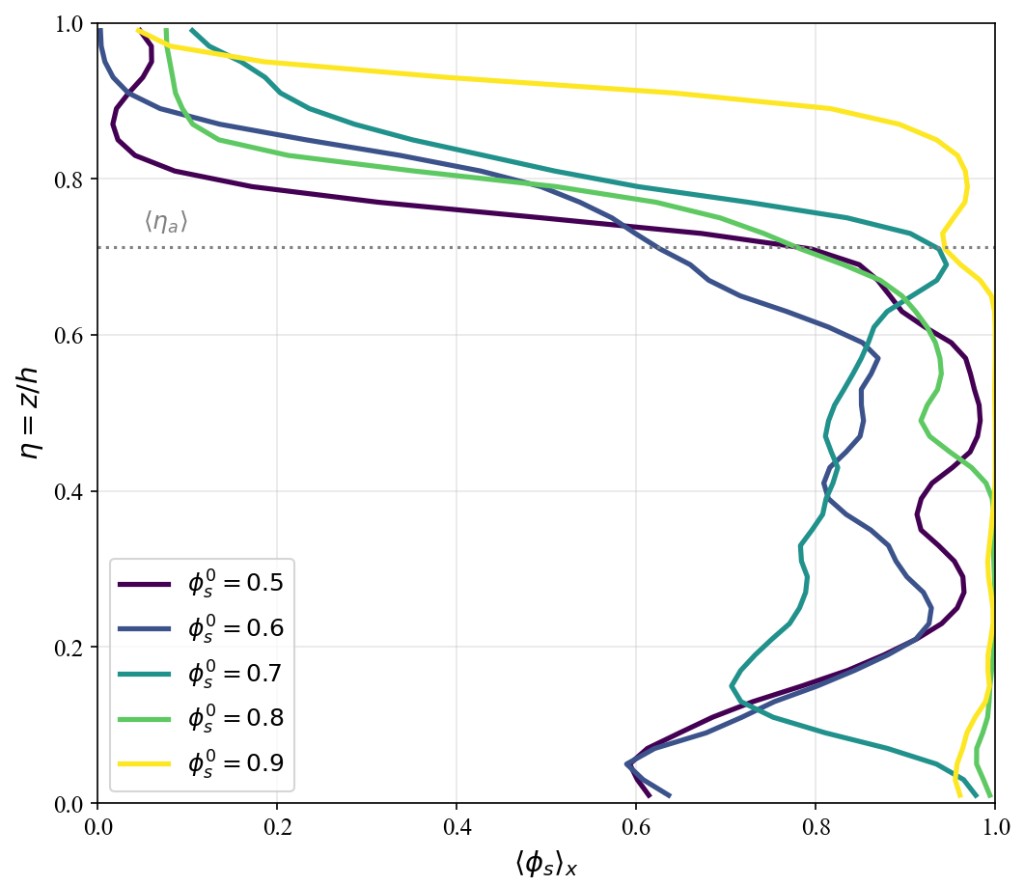
\includegraphics[width=\textwidth]{F1_panel_a_experimental.png}
        \caption{Experimental data.}
        \label{fig:F1a}
    \end{subfigure}
    \hfill
    \begin{subfigure}[t]{0.32\textwidth}
        \centering
        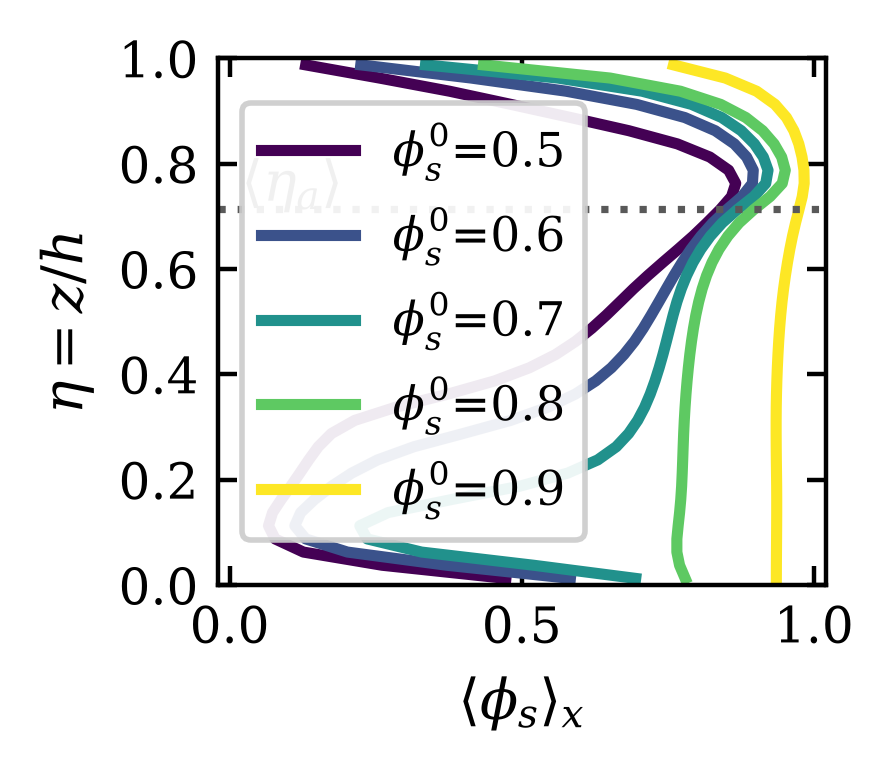
\includegraphics[width=0.28\paperwidth]{F1_panel_a_con_difusion.png}
        \caption{With granular diffusion ($A = 0.108$). Dashed curves: Gray \&
                 Chugunov (2006) equilibrium with $\ell = 0.135$\,mm.}
        \label{fig:F1b}
    \end{subfigure}
    \hfill
    \begin{subfigure}[t]{0.32\textwidth}
        \centering
        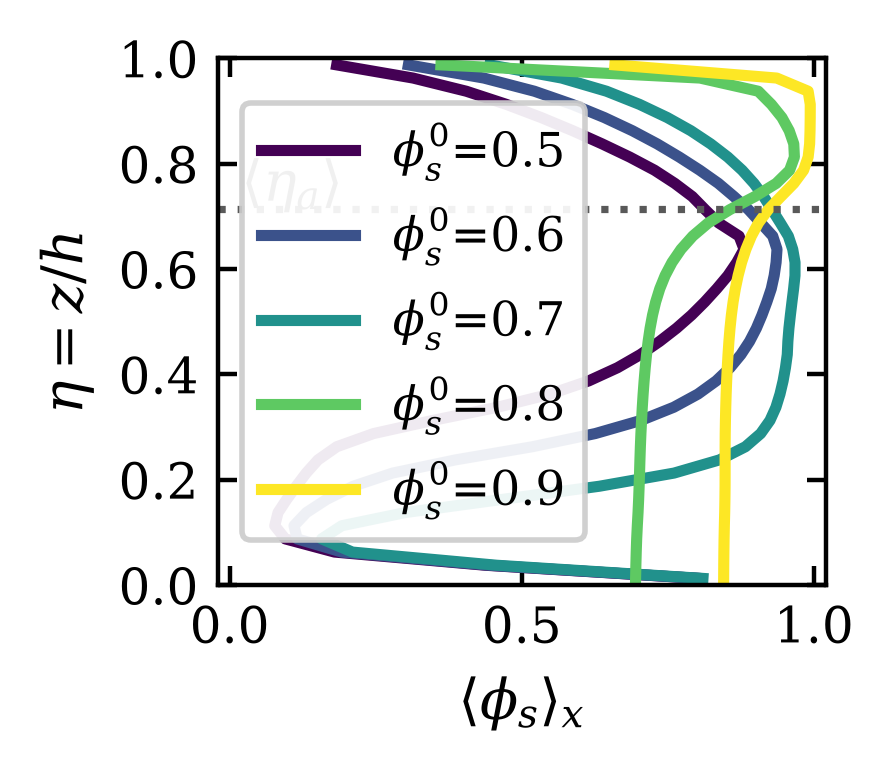
\includegraphics[width=0.28\paperwidth]{F1_panel_b_sin_difusion.png}
        \caption{Without diffusion (pure hyperbolic model): upper bound of
                 compositional contrast.}
        \label{fig:F1c}
    \end{subfigure}
    \caption{%
        \textbf{Vertical sorting profile averaged in $x$ over the dune body.}
        Panel (a) shows the experimental data. Panels (b) and (c) show the simulated profiles
        ($t = 2400$\,s, $i = 0.00975$) for five initial concentrations
        $\phi_s^0 \in \{0.5, 0.6, 0.7, 0.8, 0.9\}$.
        The horizontal dotted line marks $\langle\eta_a\rangle \approx 0.71$
        (mean roof of the buried deposit).
    }
    \label{fig:F1}
\end{figure}

\subsection*{Analysis and interpretation}

Figure~\ref{fig:F1} shows the compositional profile averaged along
the dune body for the experiment and both model configurations:

\paragraph{Panel (a) --- experimental data.}
The experimental profiles establish the physical baseline, exhibiting the characteristic three-layer pattern (coarse base, fines-rich body, and coarse surface crust) that our numerical models aim to reproduce.

\paragraph{Panel (b) --- with diffusion.}
All runs exhibit the same \textbf{three-layer} pattern, which is the
key structural signature of the segregation process:
\begin{enumerate}
    \item \textit{Base} ($\eta \lesssim 0.3$): enriched in coarse grains.
          This is a basal crust formed early, when the initial uniform mixture
          was first exposed to segregation and the coarse grains quickly settled
          before being permanently buried.
    \item \textit{Body} ($0.3 \lesssim \eta \lesssim \eta_a$): a positive
          gradient of fines upward, direct evidence of active vertical segregation
          within the mobile active layer.
    \item \textit{Surface} ($\eta \gtrsim \eta_a$): a return to low $\phi_s$
          values, forming a coarse surface crust. Segregation continually expels
          coarse grains upwards, which are re-entrained by the flow before burial.
\end{enumerate}

\subsubsection*{Physical definition of the active layer base ($\eta_a$)}
The dimensionless active layer base $\eta_a$ separates the permanently buried deposit from the actively shearing mobile layer. It is defined locally as $\eta_a(x) = 1 - \delta_a / h(x)$, where $\delta_a$ is the physical thickness of the active layer (fixed at $1.5$\,mm in the model) and $h(x)$ is the local dune height. Because the dune height $h(x)$ varies spatially, the horizontal dotted line in Figure~\ref{fig:F1} represents the spatial average over the dune body, $\langle\eta_a\rangle = \langle 1 - \delta_a / h(x) \rangle \approx 0.713$. This means that, on average, the upper $28.7\%$ of the column is actively flowing, while the bottom $71.3\%$ constitutes the frozen, buried deposit.
The dashed curves represent the theoretical equilibrium profile predicted by Gray \& Chugunov (2006) for a steady segregation--diffusion balance. In its dimensional form, the local volumetric fraction of fines $\phi_s(z)$ at a height $z$ from the bed is expressed as:
\begin{equation}
    \phi_s(z) = \frac{1}{1 + A \exp\left(\frac{f_{sl} z}{D_{sl}}\right)}
\end{equation}
where $f_{sl}$ is the maximum segregation velocity and $D_{sl}$ is the granular diffusion coefficient. Expressed in dimensionless form, scaling the height with the total flow thickness $h$ via the variable $\eta = z/h$, the equation becomes:
\begin{equation}
    \phi_s(\eta) = \frac{1}{1 + A \exp(Pe \cdot \eta)}
\end{equation}
where $Pe = \frac{f_{sl} h}{D_{sl}}$ is the segregation Péclet number (quantifying the relative strength of segregation versus diffusion), and $A$ is an integration constant determined by mass conservation. 

The function of these curves is to demonstrate that the system relaxes \textit{partially} towards this diffusive steady state within the mobile active layer, but the rapid burial of sediment downwards interrupts the segregation process before the equilibrium can be fully reached.

\paragraph{Panel (c) --- without diffusion.}
The profiles are more pronounced: the interfaces are sharper because
without $D_{sl}$ no mechanism broadens them. This panel establishes the
\textbf{upper limit} of the compositional contrast achievable in the simulated
regime, and serves as a reference to isolate the diffusion effect
(Section~\ref{sec:diffusion}). The three-layer pattern is identical in
structure, confirming that it is driven by the advective segregation flux
rather than by diffusion.

The gradation index $\langle\phi_s\rangle_{\rm top} - \langle\phi_s\rangle_{\rm bottom}$
is positive for all concentrations ($\phi_s^0 \leq 0.7$), confirming that the
deposit \textbf{fines upwards}. It decreases as $\phi_s^0$ increases, driven
by the non-linearity $\phi_s(1-\phi_s)$ of the segregation flux.
Granular diffusion reduces the index by $\approx 20\%$ without altering the
qualitative trend (Table~\ref{tab:gradation}).

\begin{table}[H]
    \centering
    \begin{tabular}{cccccc}
        \toprule
        & $\phi_s^0 = 0.5$ & $\phi_s^0 = 0.6$ & $\phi_s^0 = 0.7$
        & $\phi_s^0 = 0.8$ & $\phi_s^0 = 0.9$ \\
        \midrule
        With diffusion    & $+0.48$ & $+0.44$ & $+0.27$ & $+0.04$ & $+0.01$ \\
        Without diffusion & $+0.53$ & $+0.51$ & $+0.35$ & $+0.05$ & $+0.02$ \\
        \bottomrule
    \end{tabular}
    \caption{Gradation index
             $\langle\phi_s\rangle_{\rm top} - \langle\phi_s\rangle_{\rm bottom}$
             for the five initial concentrations.}
    \label{tab:gradation}
\end{table}

\newpage
% ============================================================
\section{Velocity Field in the Co-moving Frame and Trapped Coarse Zone}
\label{sec:velocity}
% ============================================================

The three-layer pattern identified in Section~\ref{sec:sorting} raises
the central mechanistic question: \textit{what keeps the coarse grains
trapped in the interior of the dune?} This section addresses it by
inspecting the flow field in the reference frame co-moving with the dune.

\begin{figure}[H]
    \centering
    \begin{subfigure}[b]{1.0\textwidth}
        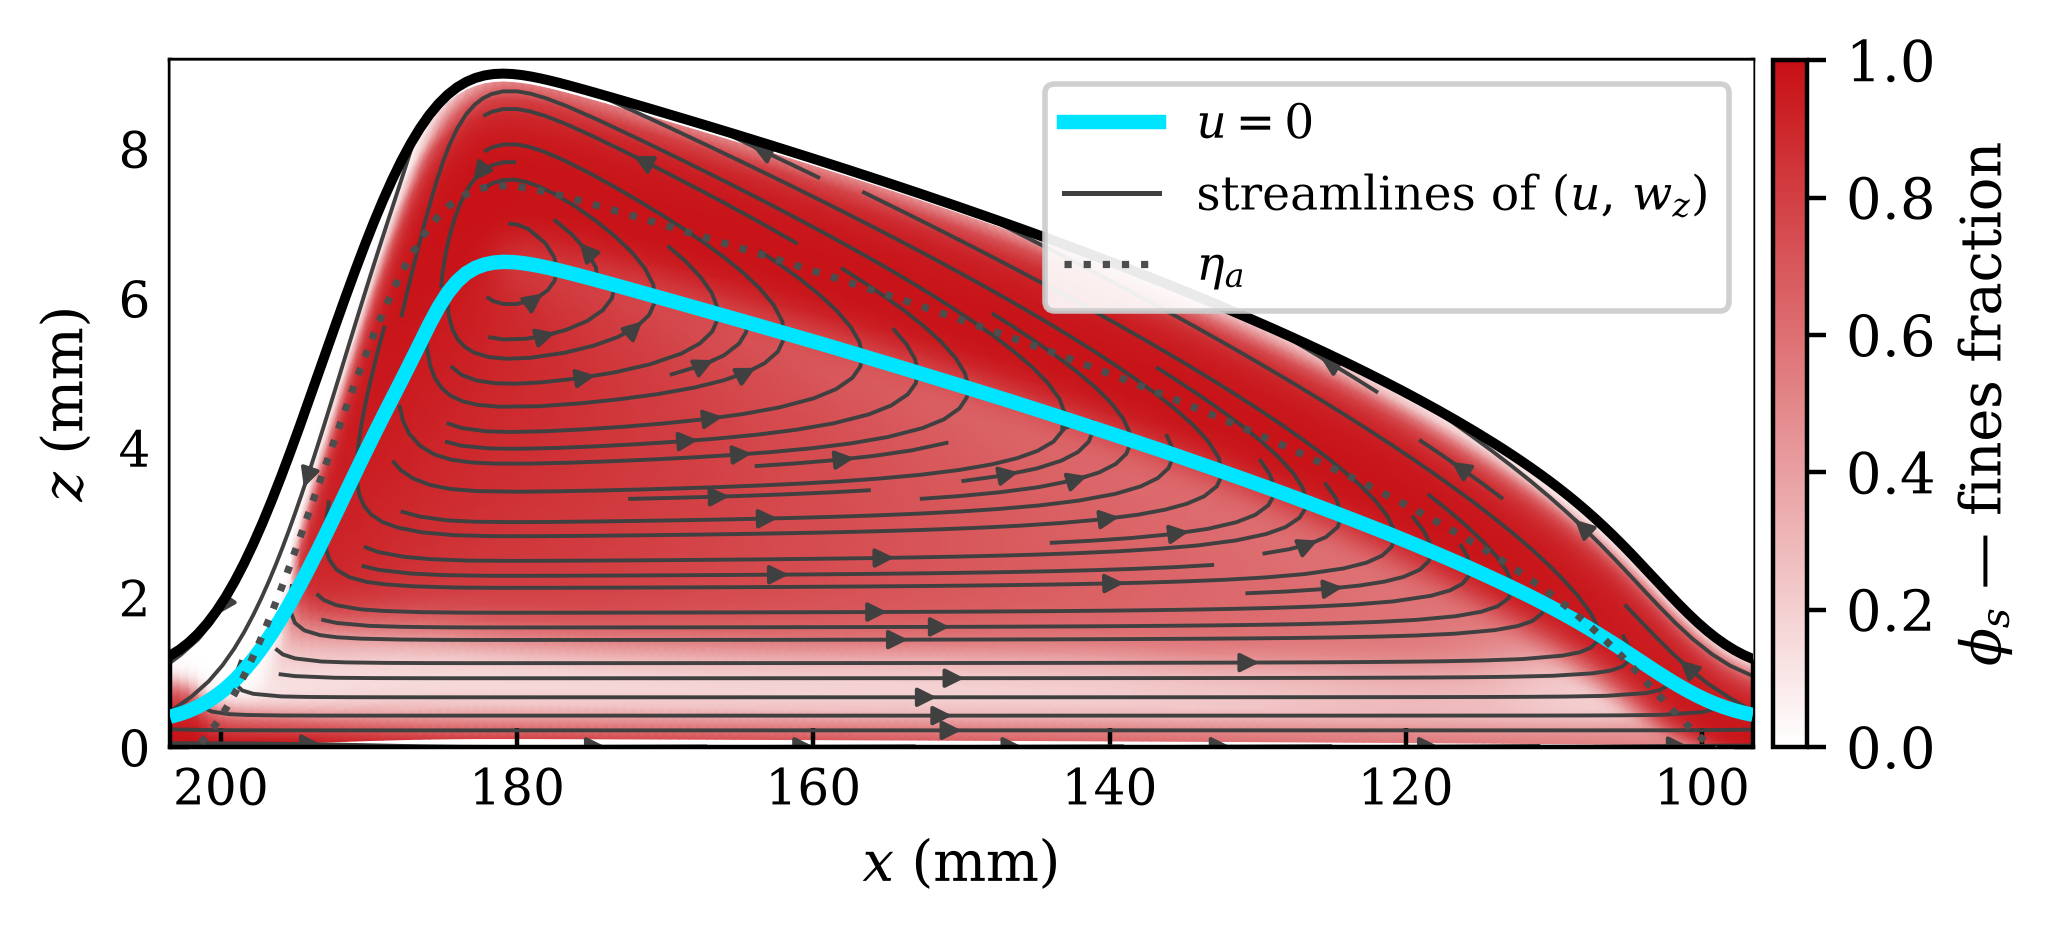
\includegraphics[width=\textwidth]{F2_panel_a.png}
    \end{subfigure}
    \vspace{0.3cm}
    
    \begin{subfigure}[b]{1.0\textwidth}
        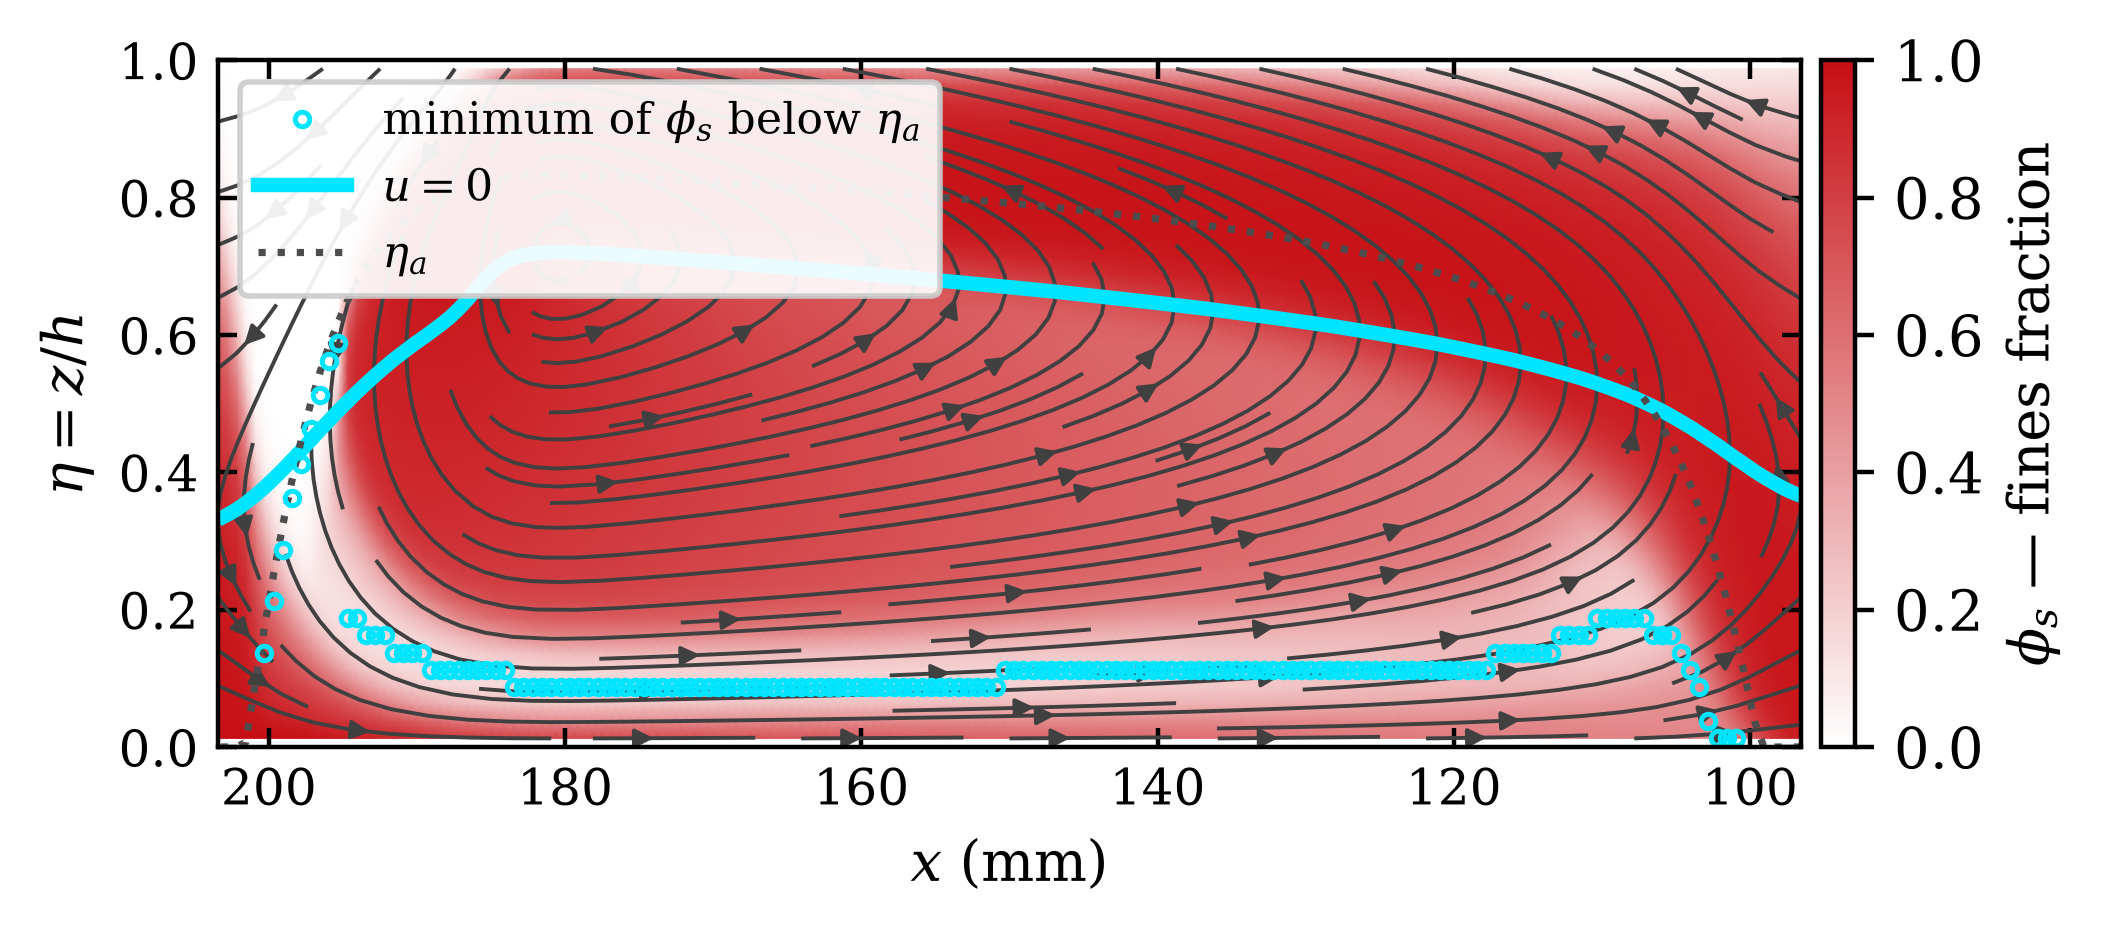
\includegraphics[width=\textwidth]{F2_panel_b.png}
    \end{subfigure}
    \caption{%
        \textbf{The trapped coarse zone and the recirculation cell}
        ($\phi_s^0 = 0.70$, with diffusion, $t = 2400$\,s).
        \textbf{(a)} Physical coordinates: $\phi_s(x,z)$, streamlines of
        $(u, w_z)$ in the co-moving frame with the dune, and isoline $u = 0$ (cyan).
        \textbf{(b)} $\sigma$-mesh (rectangular): the same field in
        coordinates $(x, \eta)$. The cyan circles mark the minimum of $\phi_s$
        below $\eta_a$ (coarse-enriched zone).
    }
    \label{fig:F2}
\end{figure}

\subsection*{Analysis and interpretation}

\paragraph{Panel (a) --- physical coordinates.}
The isoline $u = 0$ (cyan) in the co-moving frame delimits the material that
\textit{overtakes} the migrating dune from material that \textit{falls behind}
and gets permanently buried. A naive hypothesis would place the coarse
enrichment right at or below this isoline. However, the figure shows that
the coarse-rich zone (light colors in the interior) does not coincide
spatially with the $u = 0$ isoline: the ``kinematic stagnation point''
hypothesis is visually refuted.

\paragraph{Panel (b) --- $\sigma$-mesh.}
The $\sigma$ (terrain-following) coordinate system reveals the full
structure of the recirculation. Quantitative analysis confirms the spatial
mismatch:

\begin{table}[H]
    \centering
    \begin{tabular}{lc}
        \toprule
        Magnitude & Value \\
        \midrule
        $\eta(u=0) - \eta(\text{coarse})$, median & $+0.527$ \\
        Range & $[-0.098,\; +0.633]$ \\
        Equivalent in mm & $+3.27$\,mm \\
        Evaluated columns & 159 \\
        Pearson correlation & $-0.54$ \\
        \bottomrule
    \end{tabular}
    \caption{Separation between the $u=0$ isoline and the coarse core.}
    \label{tab:F2}
\end{table}

The \textbf{anti-correlation} (Pearson $= -0.54$) is the most important
result: where the $u=0$ isoline rises, the coarse core descends. The true
trapping mechanism is the \textbf{closed recirculation cell} visible in both
panels, centered at $x \approx 180$\,mm, $\eta \approx 0.55$. Sediment
that enters the cell cannot exit it within the simulation time, remaining
indefinitely confined in the interior of the dune. This is analogous to the
particle recirculation described by Thornton \& Gray (2008) for
size-segregation in dense granular flows, \emph{not} to a simple stagnation
point.

\newpage
% ============================================================
\section{Controlled Comparison: Effect of Granular Diffusion}
\label{sec:diffusion}
% ============================================================

Having established the baseline structure (Sec.~\ref{sec:sorting}) and its
physical origin (Sec.~\ref{sec:velocity}), we now isolate the contribution
of granular diffusion by directly comparing the with-diffusion and
without-diffusion runs.

\begin{figure}[H]
    \centering
    \begin{subfigure}[b]{0.8\textwidth}
        \centering
        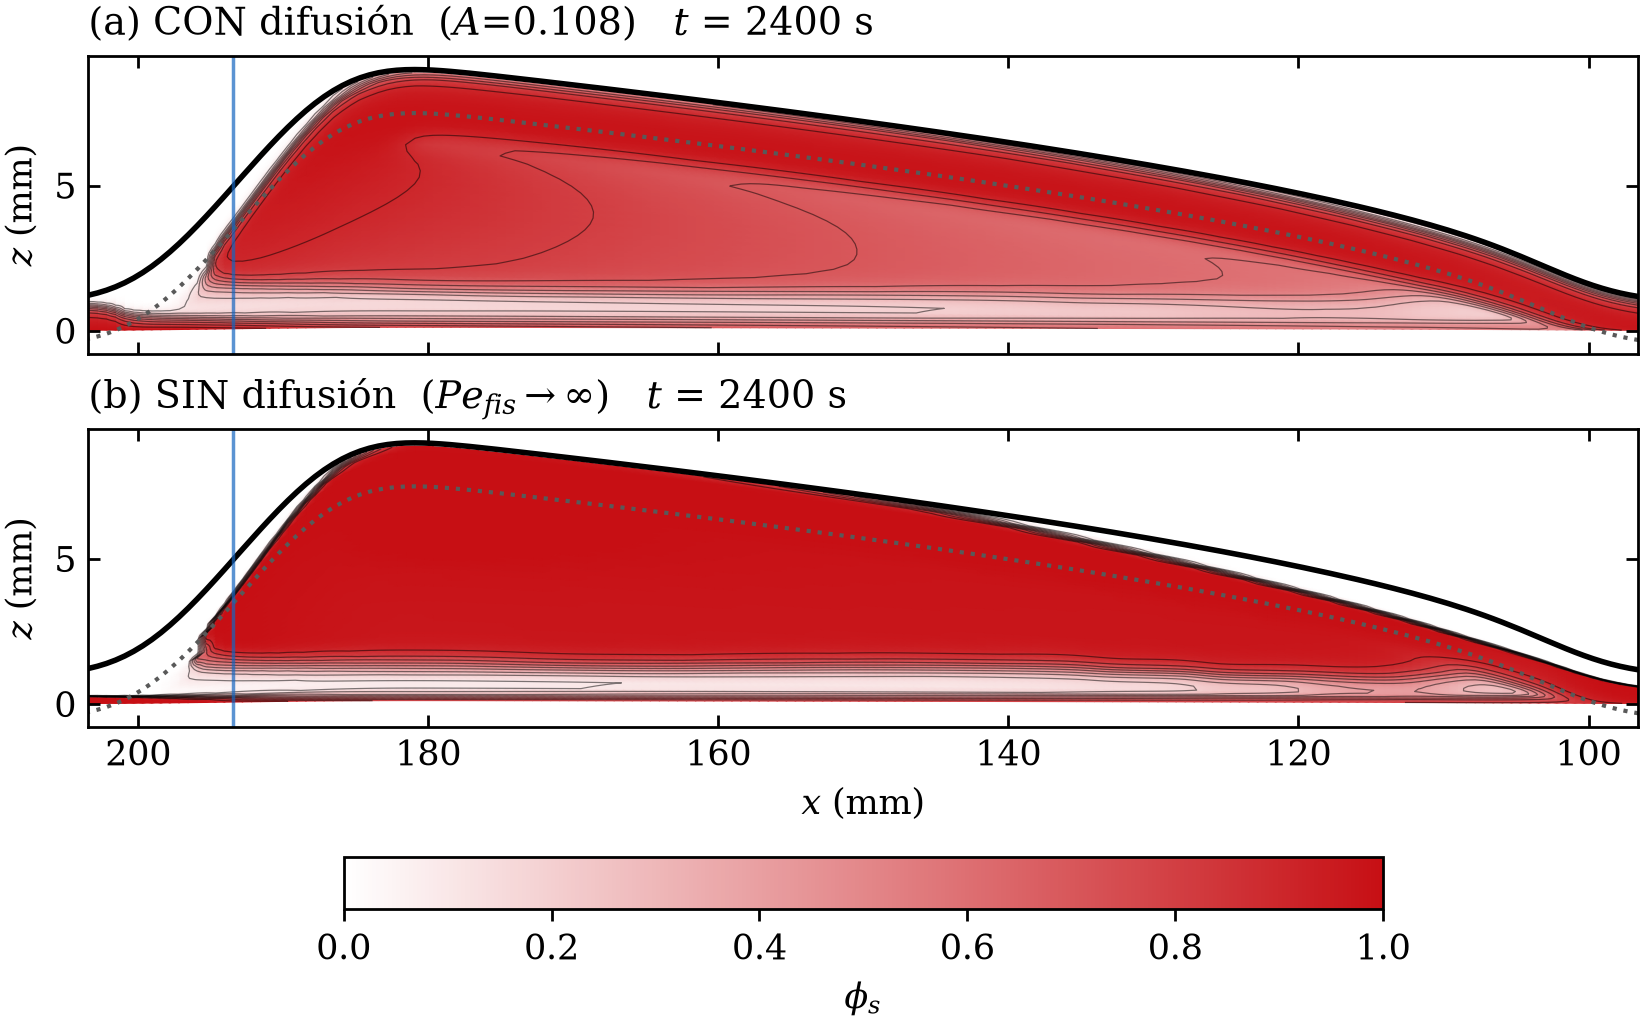
\includegraphics[width=\textwidth]{panel_ab_combinado.png}
    \end{subfigure}
    \vspace{0.5cm}
    
    \begin{subfigure}[b]{0.8\textwidth}
        \centering
        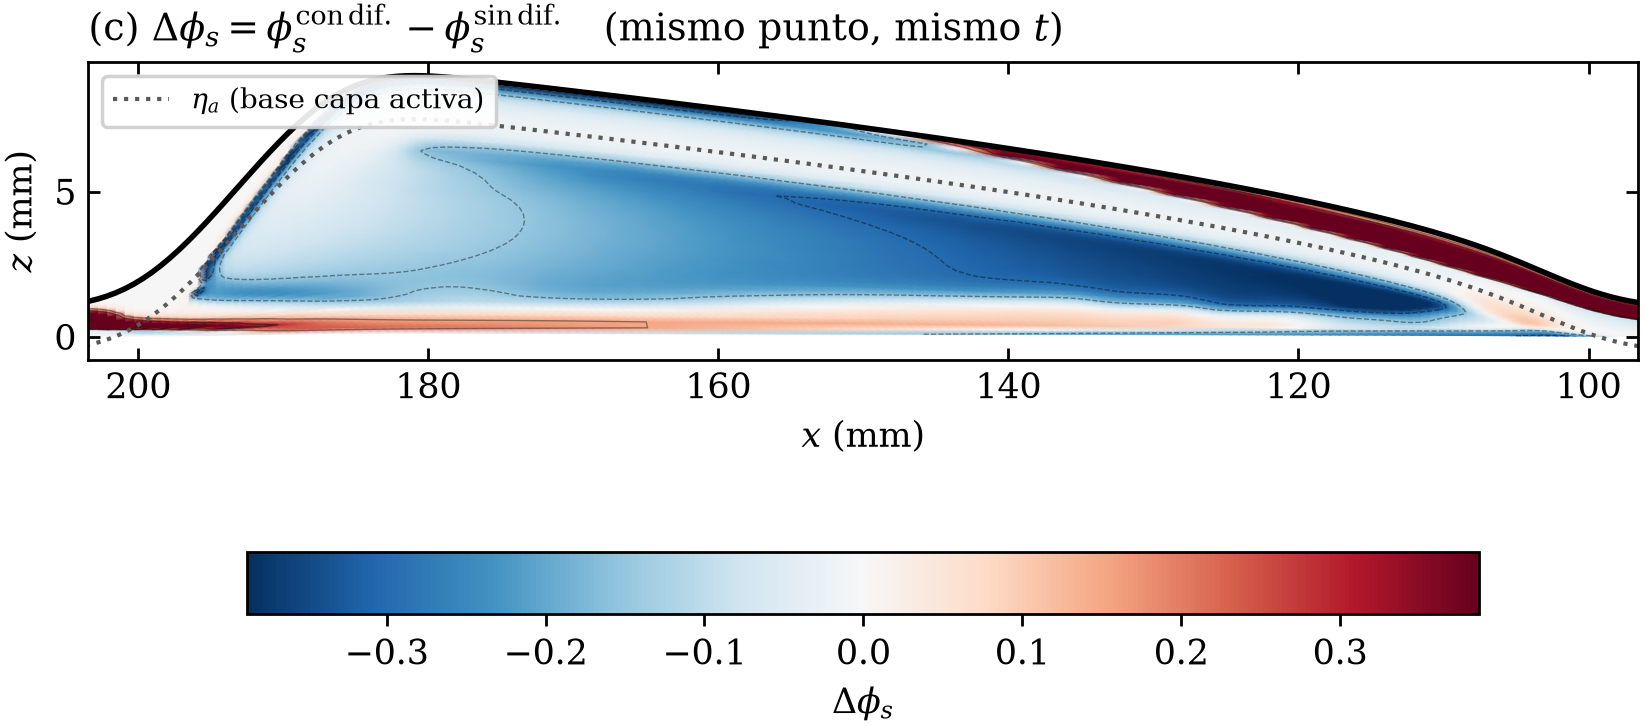
\includegraphics[width=\textwidth]{panel_c_diferencia.png}
    \end{subfigure}
    \vspace{0.5cm}

    \begin{subfigure}[b]{0.42\textwidth}
        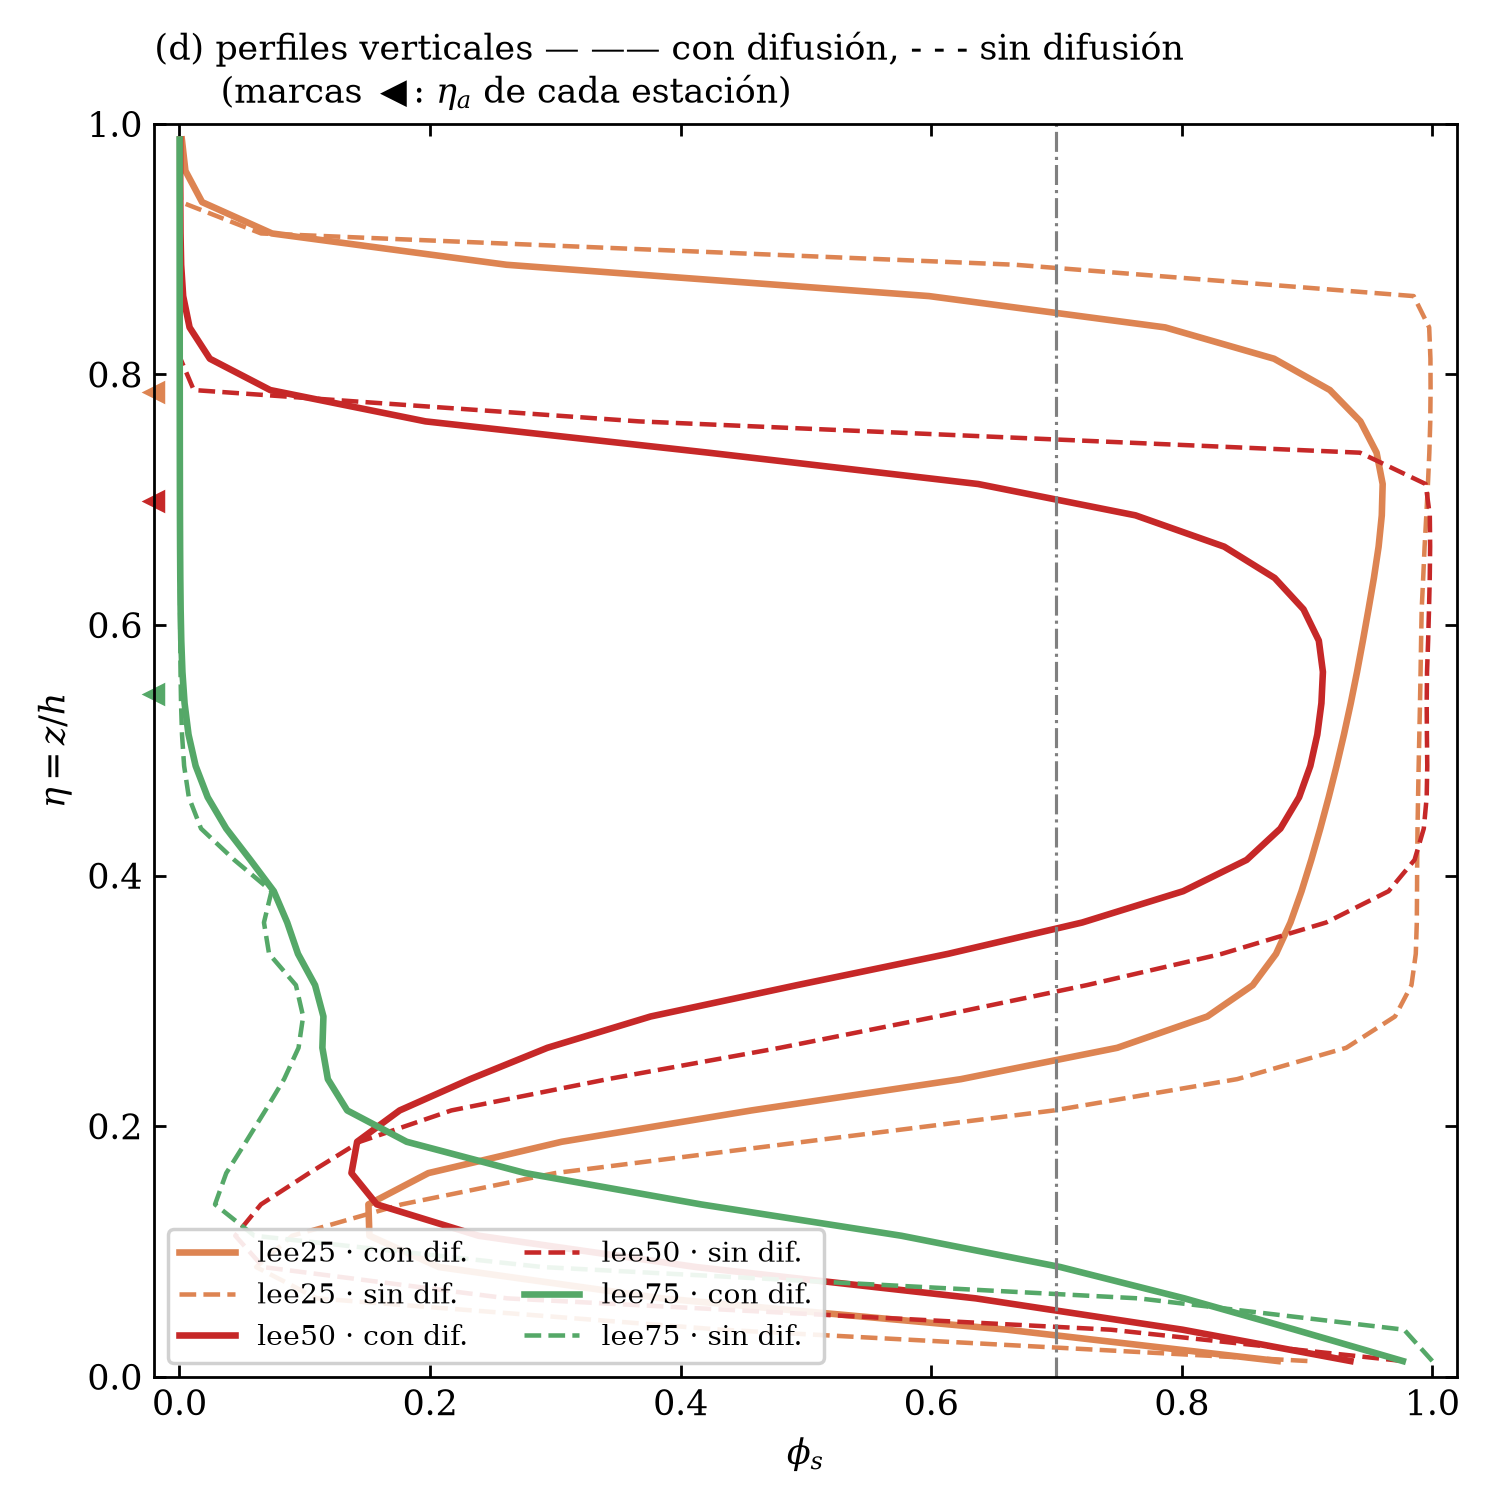
\includegraphics[width=\textwidth]{panel_d_perfiles.png}
    \end{subfigure}
    \hfill
    \begin{subfigure}[b]{0.56\textwidth}
        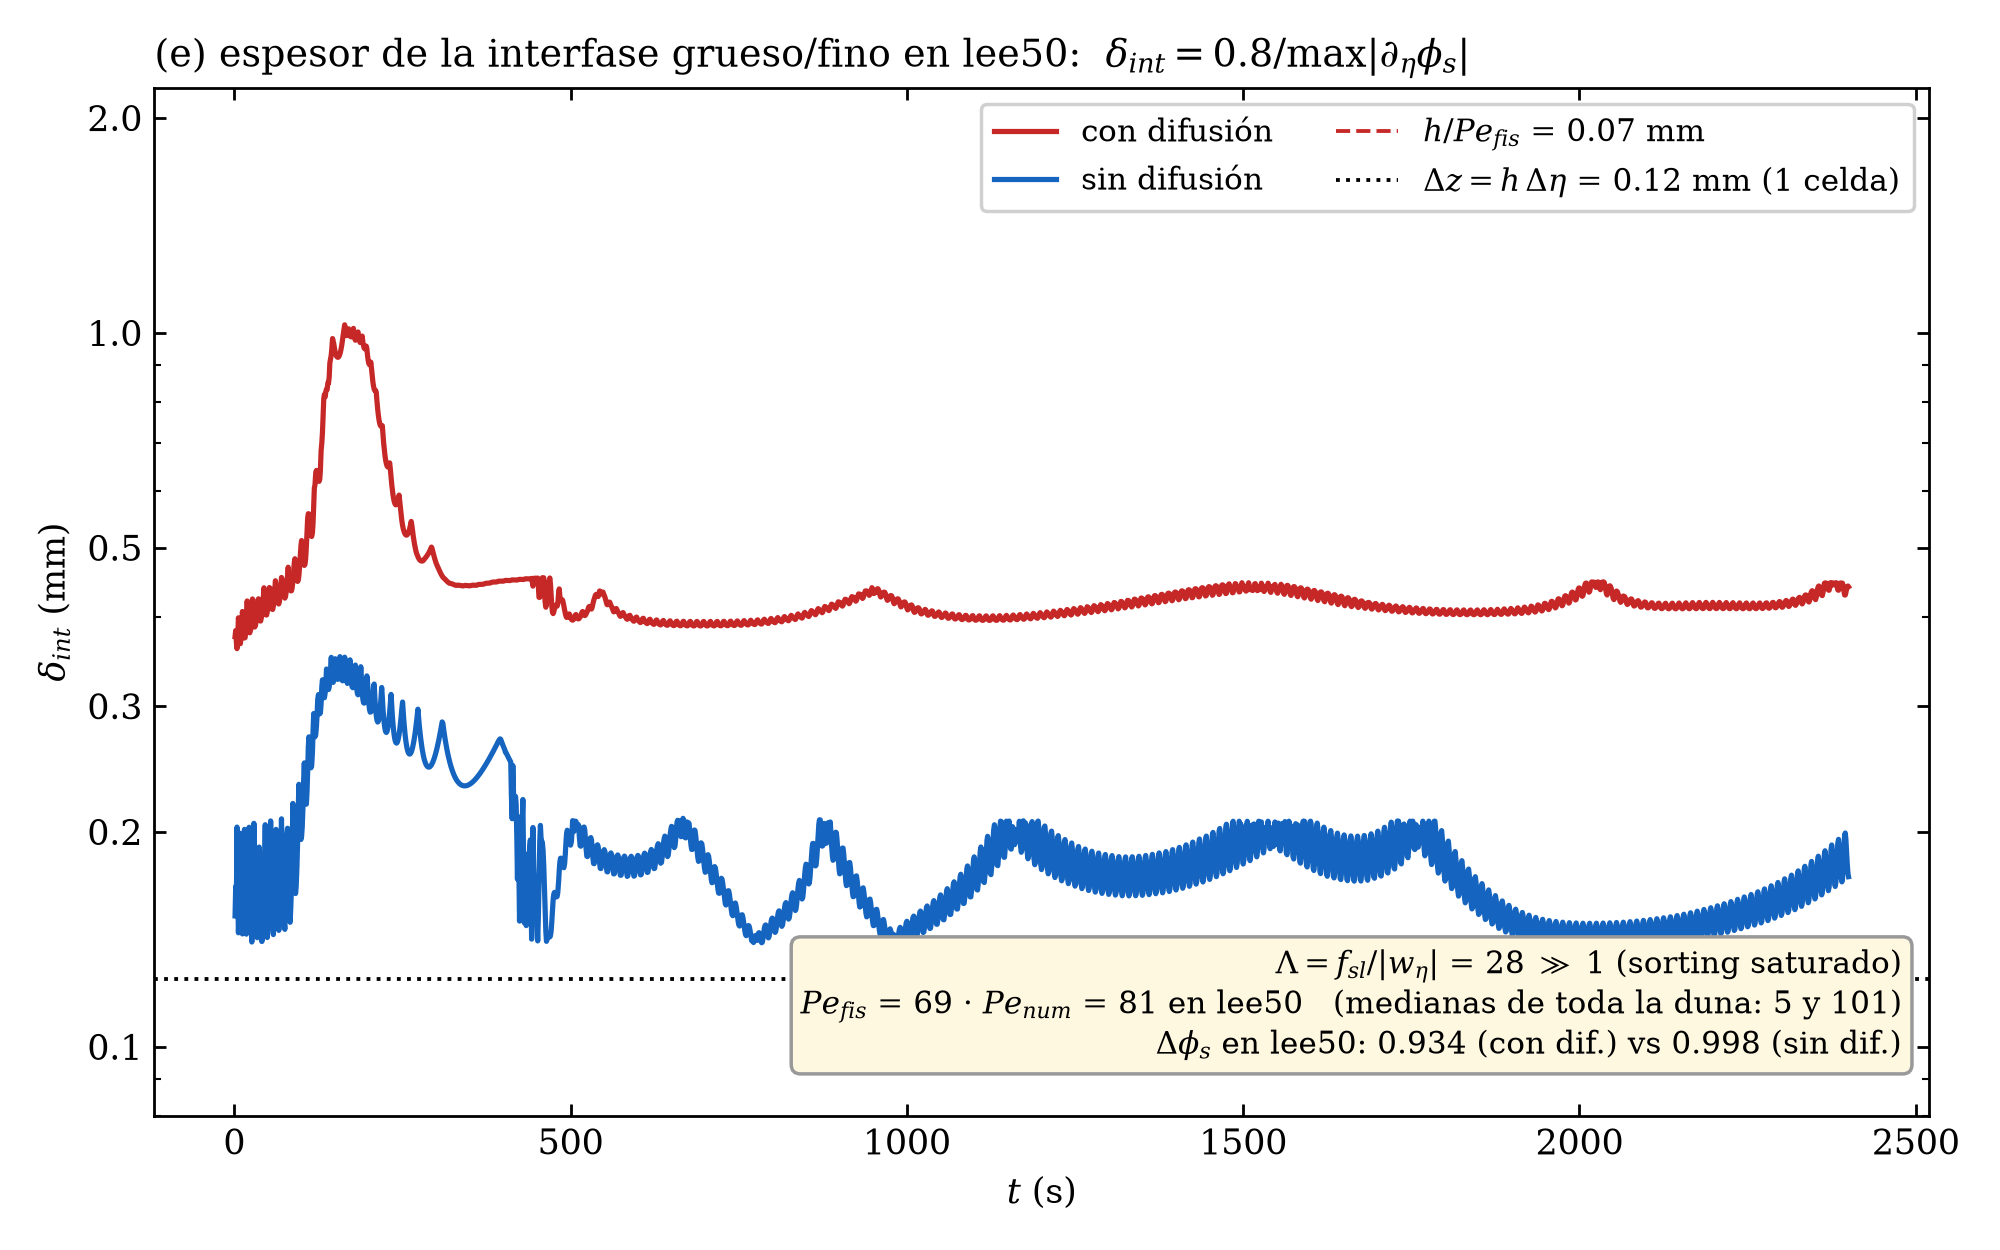
\includegraphics[width=\textwidth]{panel_e_interfase.png}
    \end{subfigure}
    
    \caption{%
        \textbf{Comparison of models with and without granular diffusion}
        ($\phi_s^0 = 0.70$, $t = 2400$\,s).
        \textbf{Top (panels a \& b):} The $\phi_s$ fields with diffusion (a) and
        without diffusion (b), displayed on the same colorscale.
        \textbf{Middle (panel c):} Pointwise difference
        $\Delta\phi_s = \phi_s^{\rm diff} - \phi_s^{\rm no\,diff}$;
        red indicates zones where diffusion adds more fines,
        blue where it adds more coarse.
        \textbf{Bottom (panels d \& e):} Vertical profiles $\langle\phi_s\rangle_x(\eta)$
        comparing both models (d) and the temporal evolution of the
        coarse/fine interface thickness $\delta_{\rm int}$ (e).
    }
    \label{fig:comp_diffusion}
\end{figure}

\subsection*{Analysis and interpretation}

Figure~\ref{fig:comp_diffusion} isolates the effect of the granular diffusion
term by a direct controlled comparison.

\begin{itemize}
    \item \textbf{Panels (a) and (b) --- global structure:} The overall layout
          of the recirculation cell, the three-layer stratification, and the
          coarse core position are essentially identical in both models. This
          demonstrates that the \emph{topology} of the segregation pattern is
          dominated by the advective segregation flux, not by diffusion.
          Diffusion is a perturbative, not a structurally dominant, process.

    \item \textbf{Panel (c) --- pointwise difference:} The difference
          $\Delta\phi_s$ is concentrated at the compositional interfaces
          (boundaries of the layers identified in Sec.~\ref{sec:sorting}),
          where diffusion broadens the transitions. Key metrics:
          \begin{itemize}
              \item \textbf{RMS} of $\Delta\phi_s$: $0.277$
              \item \textbf{Max} $|\Delta\phi_s|$: $0.944$
              \item \textbf{Color scale saturated at} $\pm0.39$
              \item $|\Delta\phi_s| > 0.05$ in $71\%$ of the dune volume.
          \end{itemize}

    \item \textbf{Panel (d) --- averaged profiles:} Diffusion reduces the
          gradation index by $\approx 20\%$ (consistent with
          Table~\ref{tab:gradation}) but does not change the sign or the
          qualitative shape of the profile.

    \item \textbf{Panel (e) --- interface thickness:} This panel provides
          the most direct evidence for the physical role of diffusion.
          The thickness $\delta_{\text{int}}$ is defined based on the maximum concentration gradient as:
          \begin{equation}
              \delta_{\text{int}} = h \frac{0.8}{\max \left| \frac{\partial \phi_s}{\partial \eta} \right|}
          \end{equation}
          This formula represents the spatial width of a linear ramp spanning $80\%$ of the composition change (from $\phi_s = 0.1$ to $0.9$). Evaluating the $10\%$--$90\%$ interval is a standard physical convention that isolates the primary transition core, avoiding the infinitely long asymptotic tails characteristic of diffusive profiles.
          Without diffusion (blue curve), the interface collapses toward
          the numerical mesh limit ($\approx 0.19$\,mm, $\sim$1.5 cells).
          With diffusion (red curve), the thickness stabilizes smoothly
          above the numerical floor at $\approx 0.45$\,mm, consistent
          with the static equilibrium $\ell \approx 0.07$\,mm modified
          by advective stretching during burial. This validates that
          the modeled broadening is a real physical effect, not a grid artifact.
\end{itemize}

\subsubsection*{Physical interpretation: the sorting front}

The \textbf{sorting front} is defined as the boundary below which the
segregation process has substantially modified the initial uniform mixture
($|\phi_s - \phi_s^0| > 0.05$). Its dynamics explain why the system
reaches the final state it does:
\begin{enumerate}
    \item \textbf{Rapid descent} ($t \lesssim 300$\,s): The front
          descends from the surface (active layer) into the dune interior
          faster than the burial rate, because the downward flux of fines
          by gravity augments the passive burial velocity.
    \item \textbf{Physical arrest} ($t \approx 300$\,s): The front
          reaches the impermeable base ($\eta = 0$). From this point, the
          entire column has been visited by segregation and no virgin sediment
          remains. The simulation then runs to $t = 2400$\,s to capture the
          slower spatial reorganization that builds the recirculation cell
          (Sec.~\ref{sec:velocity}).
\end{enumerate}

\subsubsection*{Temporal Evolution of the Interface Difference}

To further illustrate how diffusion broadens the interfaces dynamically, we track the pointwise difference $\Delta\phi_s$ over time. Figure~\ref{fig:diff_evol} shows this temporal evolution across the dune, alongside a detailed zoom of the vertical profile at the center of the avalanche face.

\begin{figure}[H]
    \centering
    \begin{subfigure}[b]{1.0\textwidth}
        \centering
        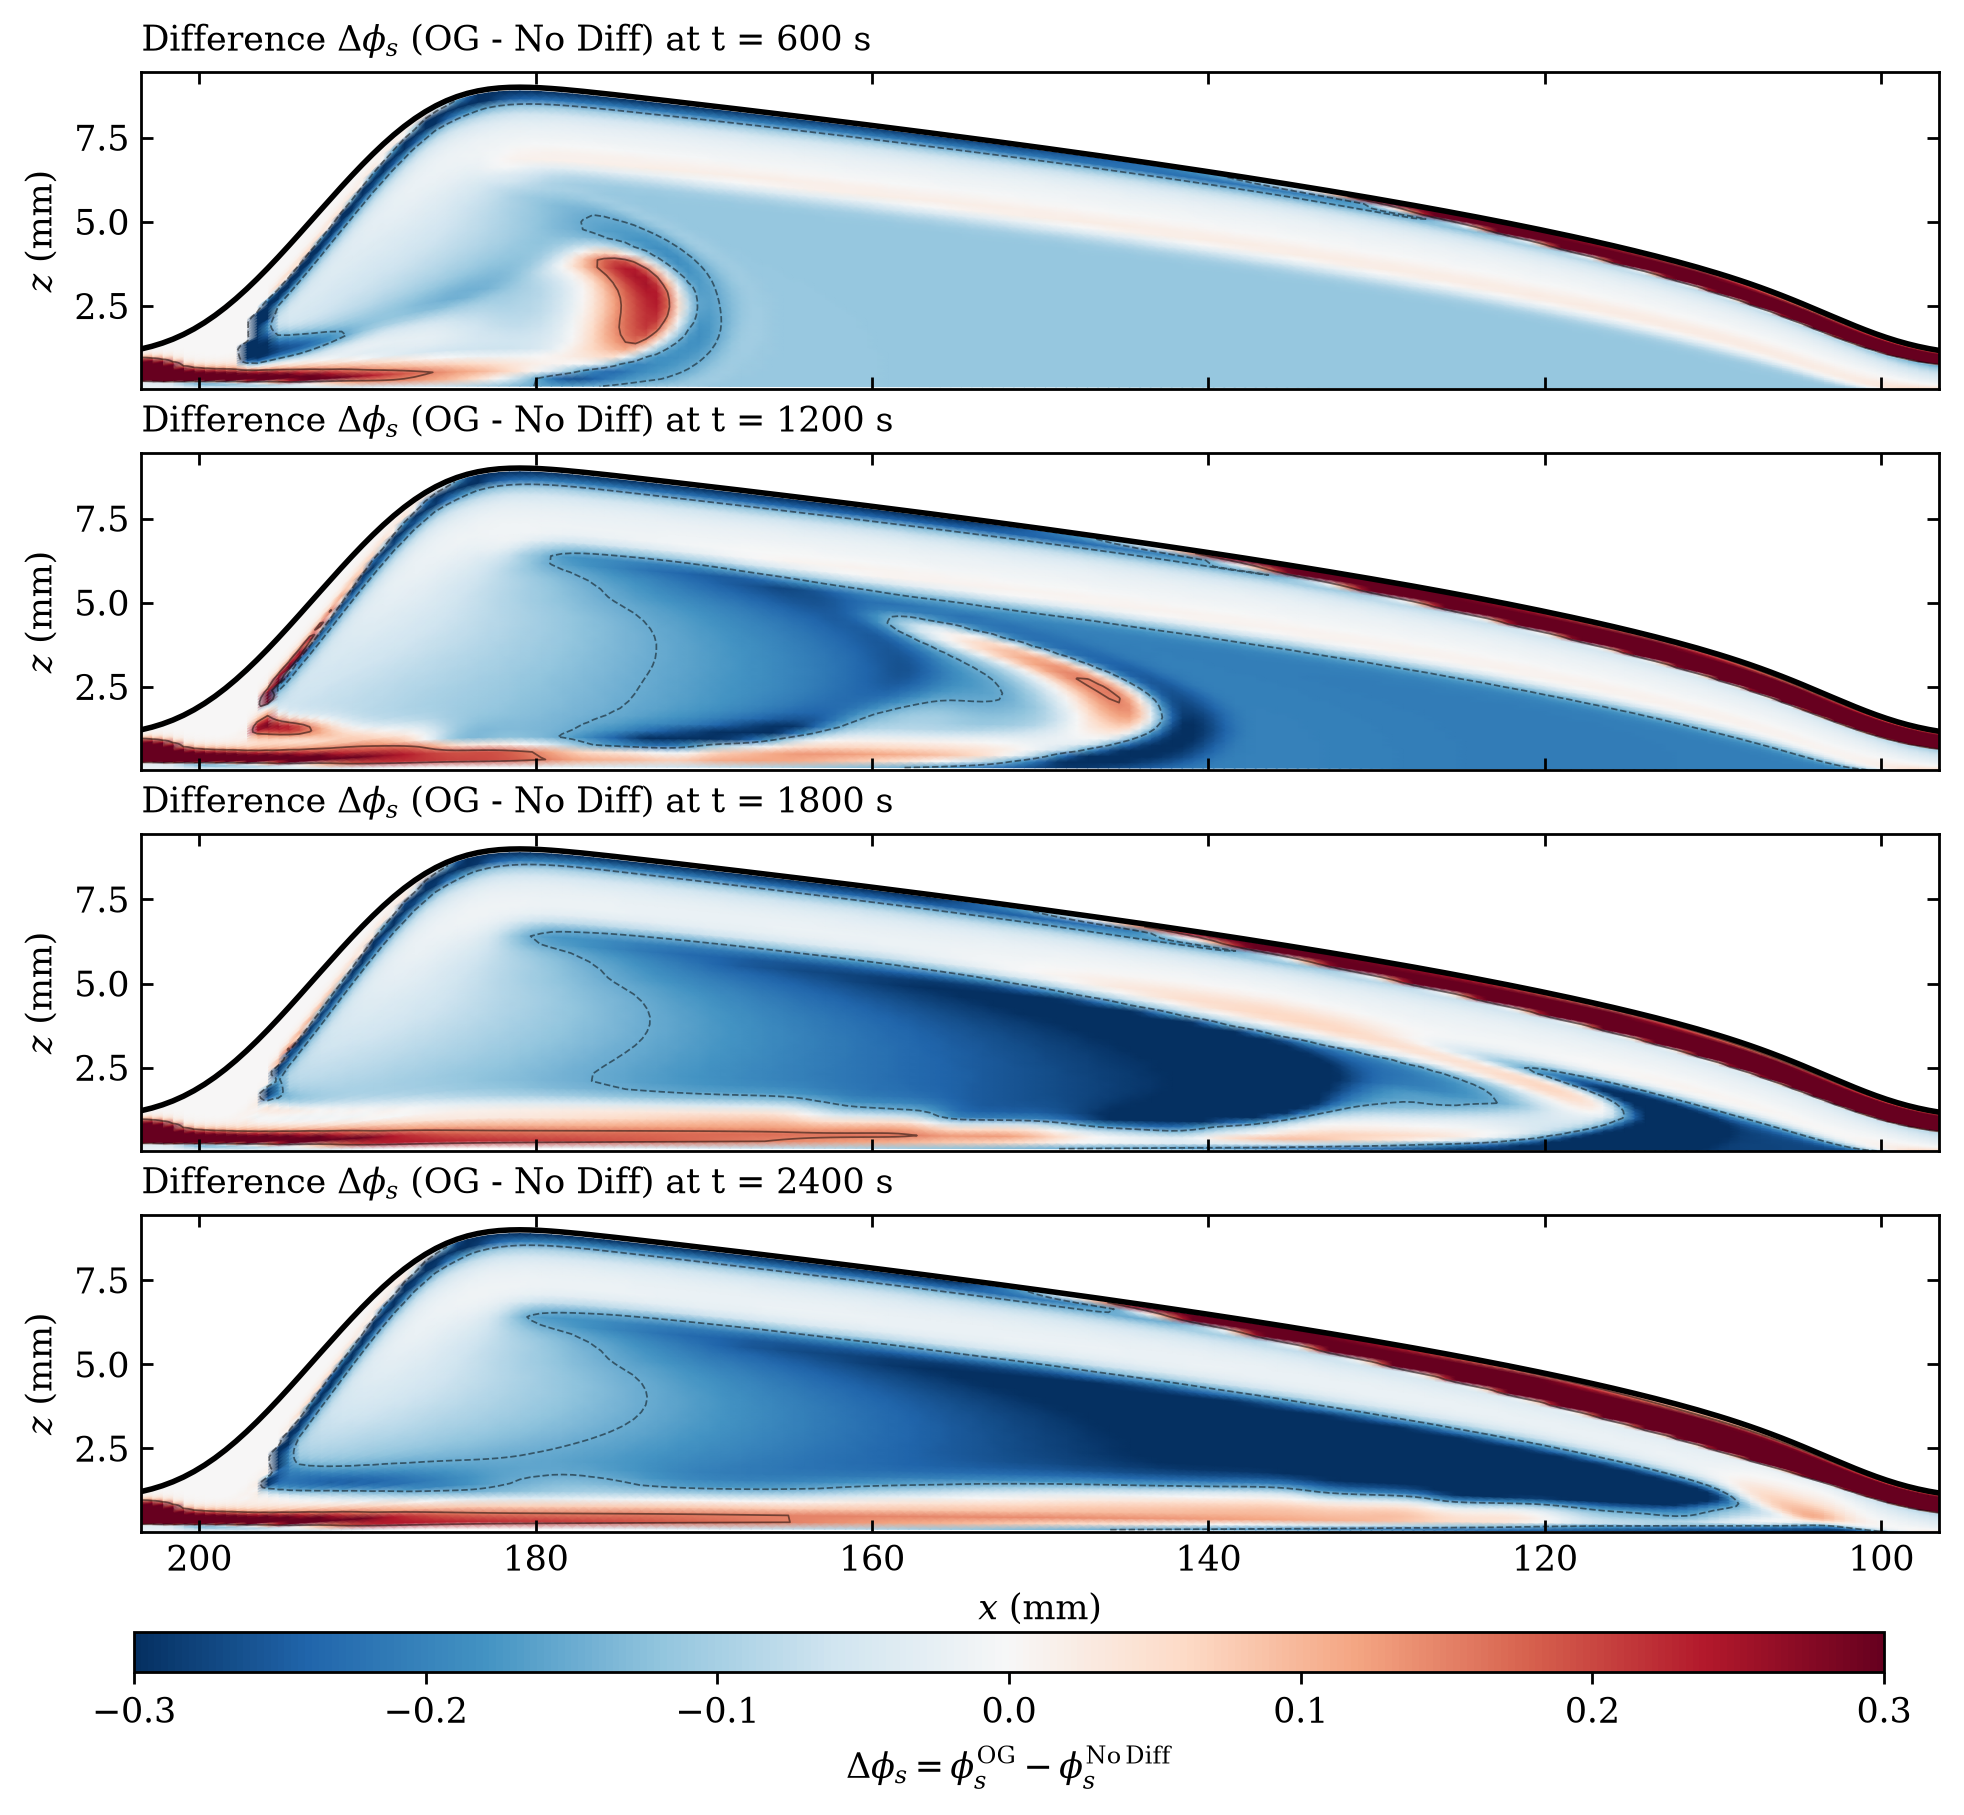
\includegraphics[width=\textwidth]{evolucion_diferencia_OG_vs_nodiff.png}
        \caption{Spatial maps of the difference $\Delta\phi_s$ at successive times.}
        \label{fig:diff_evol_maps}
    \end{subfigure}
    
    \vspace{0.5cm}
    \begin{subfigure}[b]{1.0\textwidth}
        \centering
        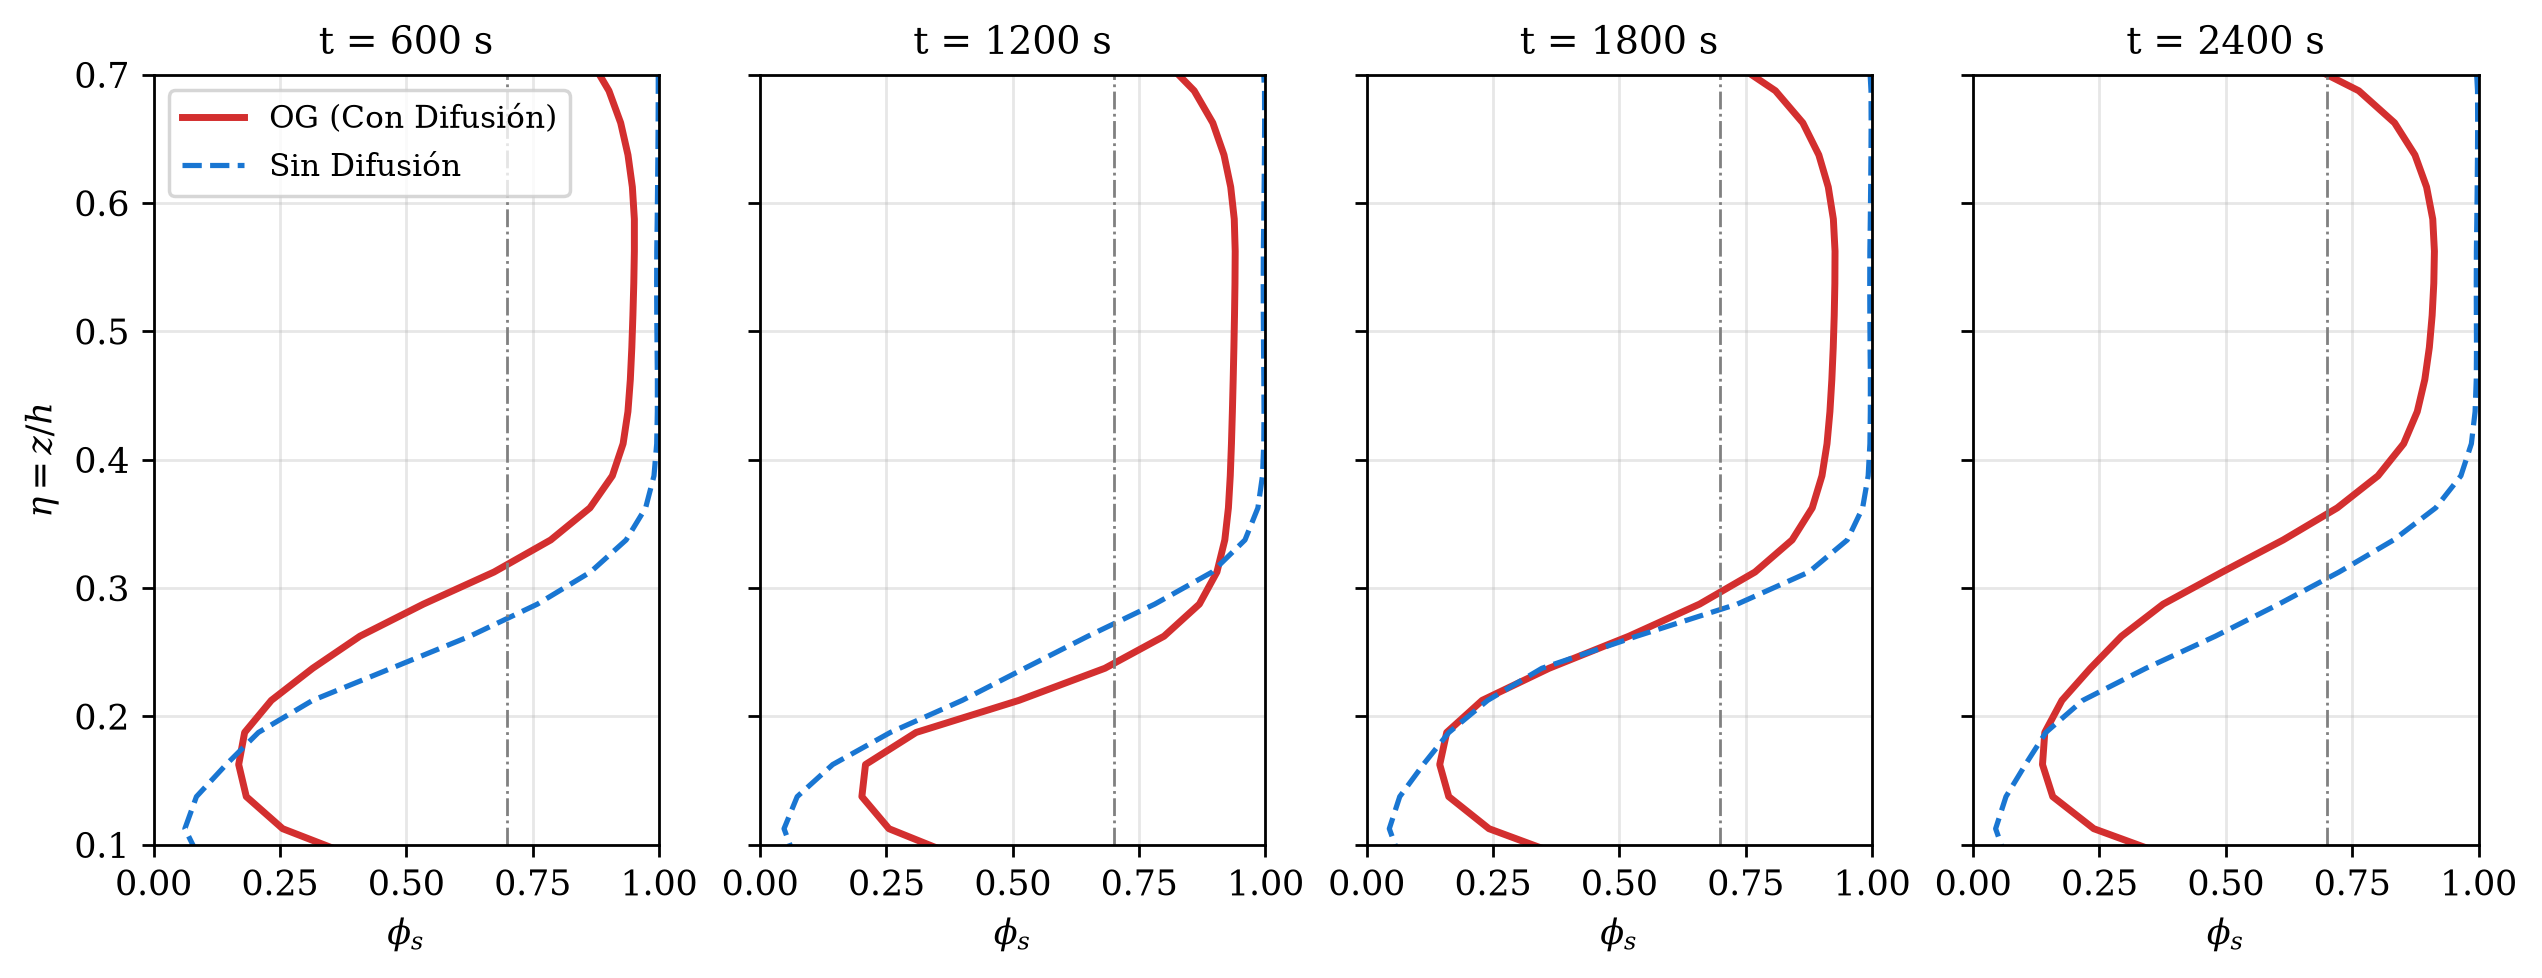
\includegraphics[width=\textwidth]{evolucion_perfiles_zoom.png}
        \caption{Zoomed vertical profiles of $\phi_s$ at the \texttt{lee50} station, highlighting the interface thickness.}
        \label{fig:diff_evol_zoom}
    \end{subfigure}
    
    \caption{%
        \textbf{Temporal evolution of the difference between the models with and without diffusion}. The maps (a) track how the broadened interfaces propagate downwards over time, while the zoomed vertical profiles (b) contrast the smooth physical transition of the OG model (red) against the abrupt step of the hyperbolic model (blue dashed line).
    }
    \label{fig:diff_evol}
\end{figure}

Table~\ref{tab:delta_int} quantifies this evolution at the \texttt{lee50} station, extracted directly from the data of Figure~\ref{fig:comp_diffusion}(e). The purely hyperbolic model (without diffusion) collapses quickly towards the numerical resolution limit (oscillating around $\approx 0.17$--$0.19$\,mm, which corresponds to $\sim 1.5$ grid cells), whereas the model with granular diffusion stabilizes the interface physically, maintaining a thickness systematically above $0.4$\,mm during the late stages of segregation.

\begin{table}[H]
    \centering
    \begin{tabular}{ccc}
        \toprule
        Time (s) & $\delta_{\text{int}}$ With Diffusion (mm) & $\delta_{\text{int}}$ Without Diffusion (mm) \\
        \midrule
        100 & 0.512 & 0.197 \\
        300 & 0.476 & 0.259 \\
        600 & 0.396 & 0.185 \\
        900 & 0.419 & 0.175 \\
        1200 & 0.403 & 0.177 \\
        1500 & 0.439 & 0.180 \\
        1800 & 0.405 & 0.171 \\
        2100 & 0.413 & 0.142 \\
        2400 & 0.441 & 0.173 \\
        \bottomrule
    \end{tabular}
    \caption{Temporal evolution of the interface thickness $\delta_{\text{int}}$ measured at the \texttt{lee50} station.}
    \label{tab:delta_int}
\end{table}

\newpage
% ============================================================
\section{Temporal Evolution of $\phi_s$: Kinetics of Vertical Sorting}
\label{sec:temporal}
% ============================================================

The fan (Sec.~\ref{sec:fan}) and the final averaged profile
(Sec.~\ref{sec:sorting}) frame the beginning and end states. Here we focus
on the \emph{path} between them: how the vertically averaged profile
$\langle\phi_s\rangle_x(\eta)$ evolves in time, and how diffusion alters
that path.

\begin{figure}[H]
    \centering
    \begin{subfigure}[t]{0.48\textwidth}
        \centering
        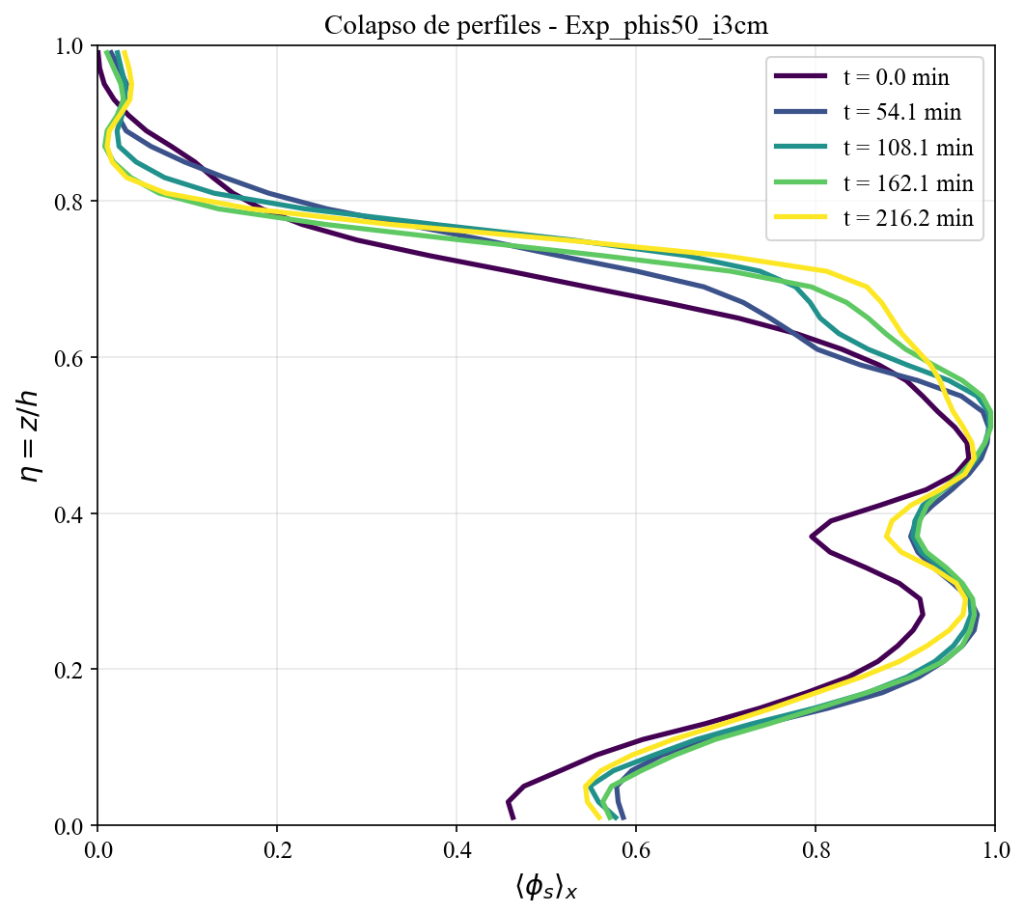
\includegraphics[width=\textwidth]{Exp_phis50_time.png}
        \caption{Experimental}
    \end{subfigure}
    \hfill
    \begin{subfigure}[t]{0.48\textwidth}
        \centering
        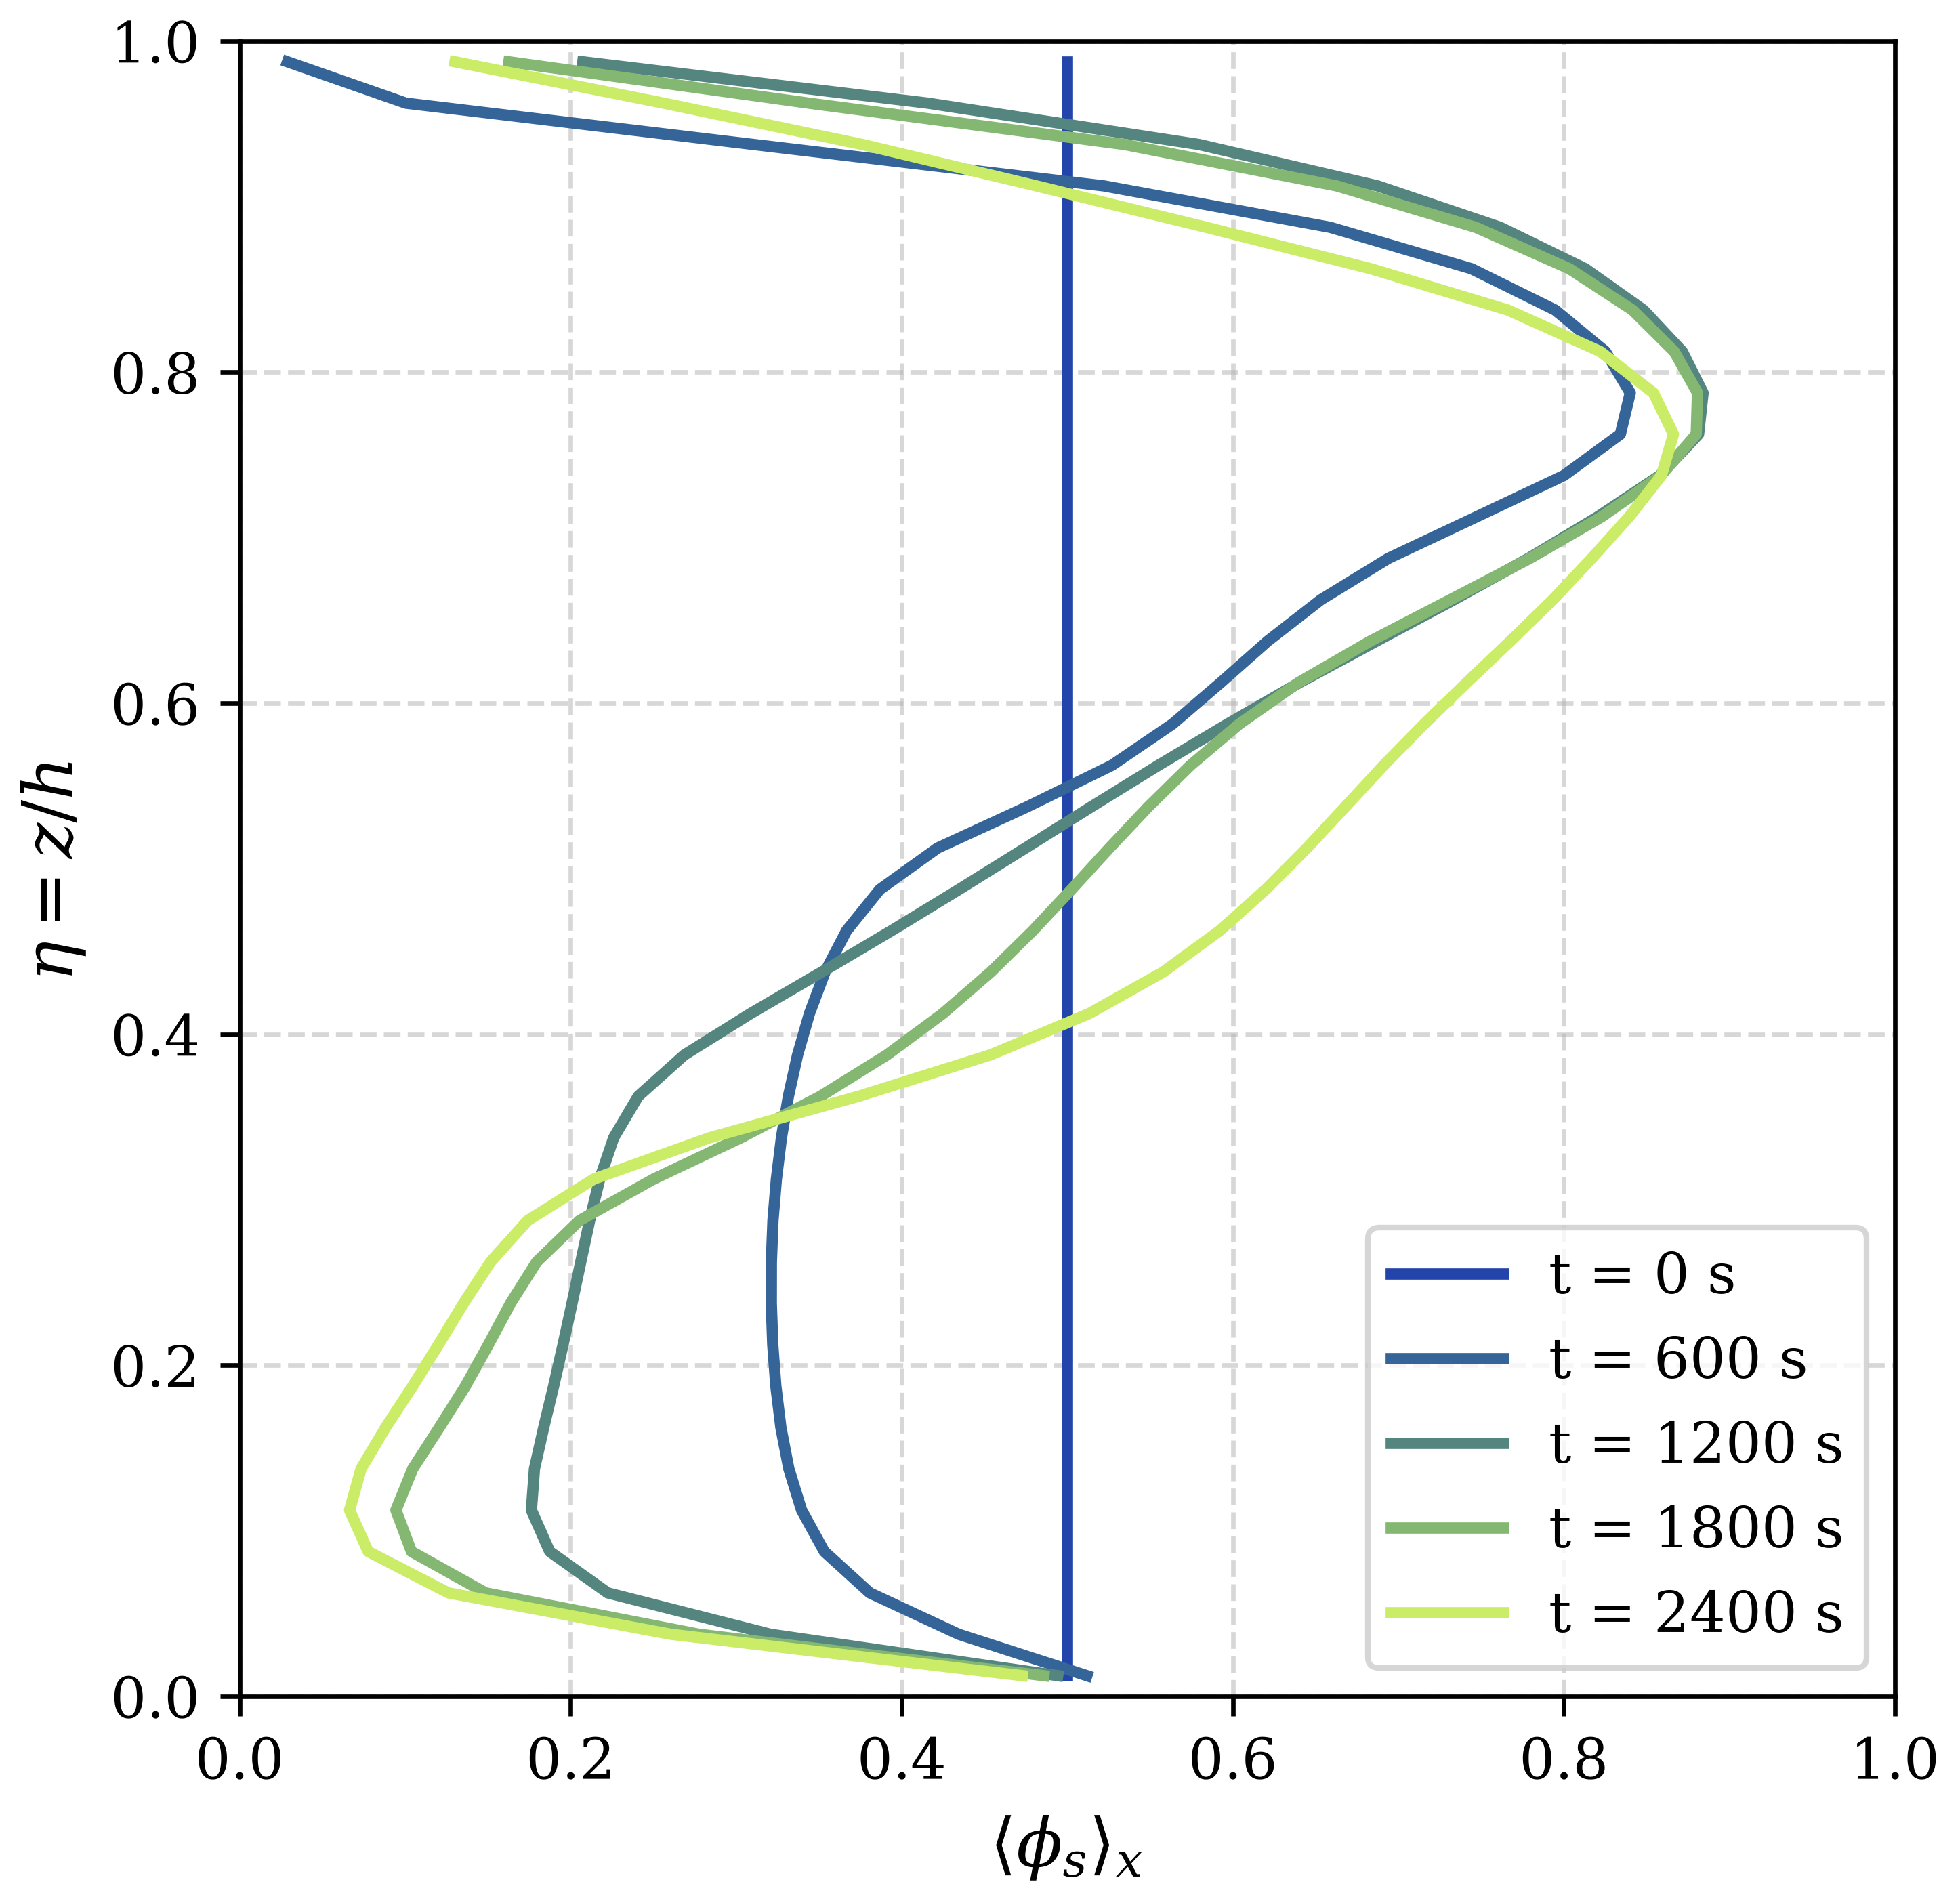
\includegraphics[width=\textwidth]{phi_s_vs_eta_time_phi50.png}
        \caption{Model}
    \end{subfigure}
    \caption{\textbf{Temporal evolution of the vertical sorting for $\phi_s^0 = 0.50$}. Left: Experimental data. Right: Model prediction.}
    \label{fig:phi50_time}
\end{figure}

\begin{figure}[H]
    \centering
    \begin{subfigure}[t]{0.48\textwidth}
        \centering
        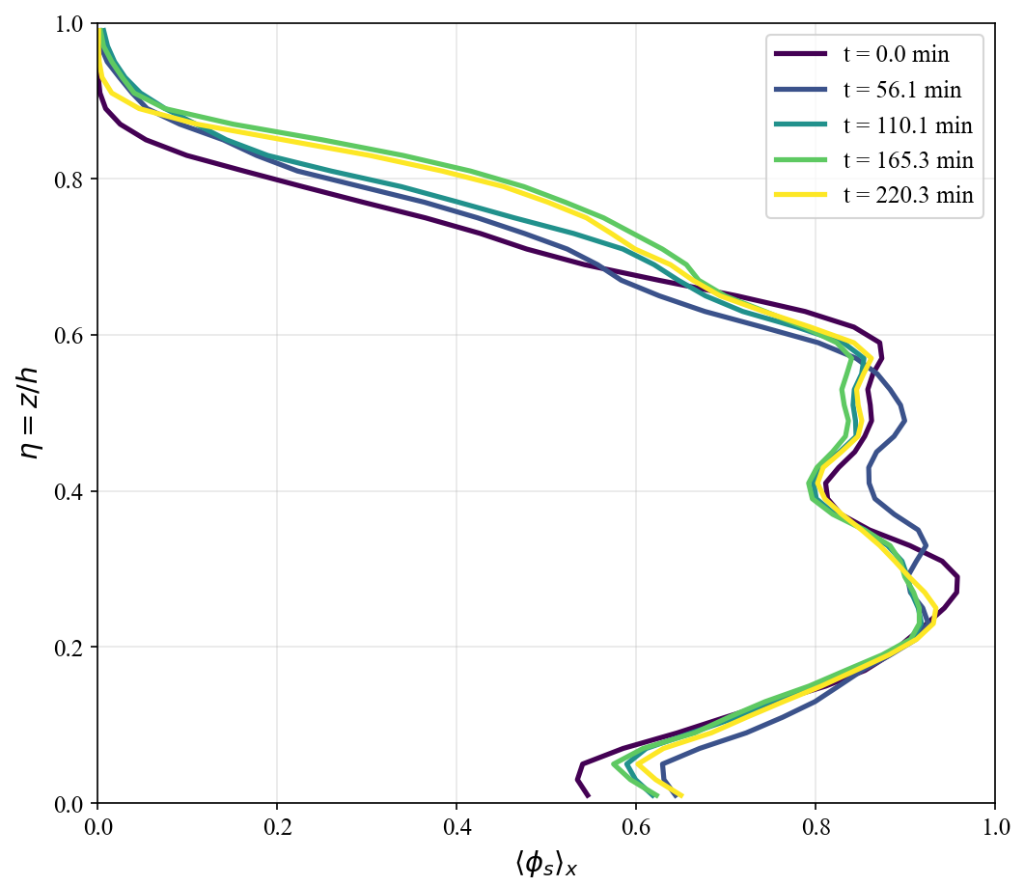
\includegraphics[width=\textwidth]{Exp_phis60_time.png}
        \caption{Experimental}
    \end{subfigure}
    \hfill
    \begin{subfigure}[t]{0.48\textwidth}
        \centering
        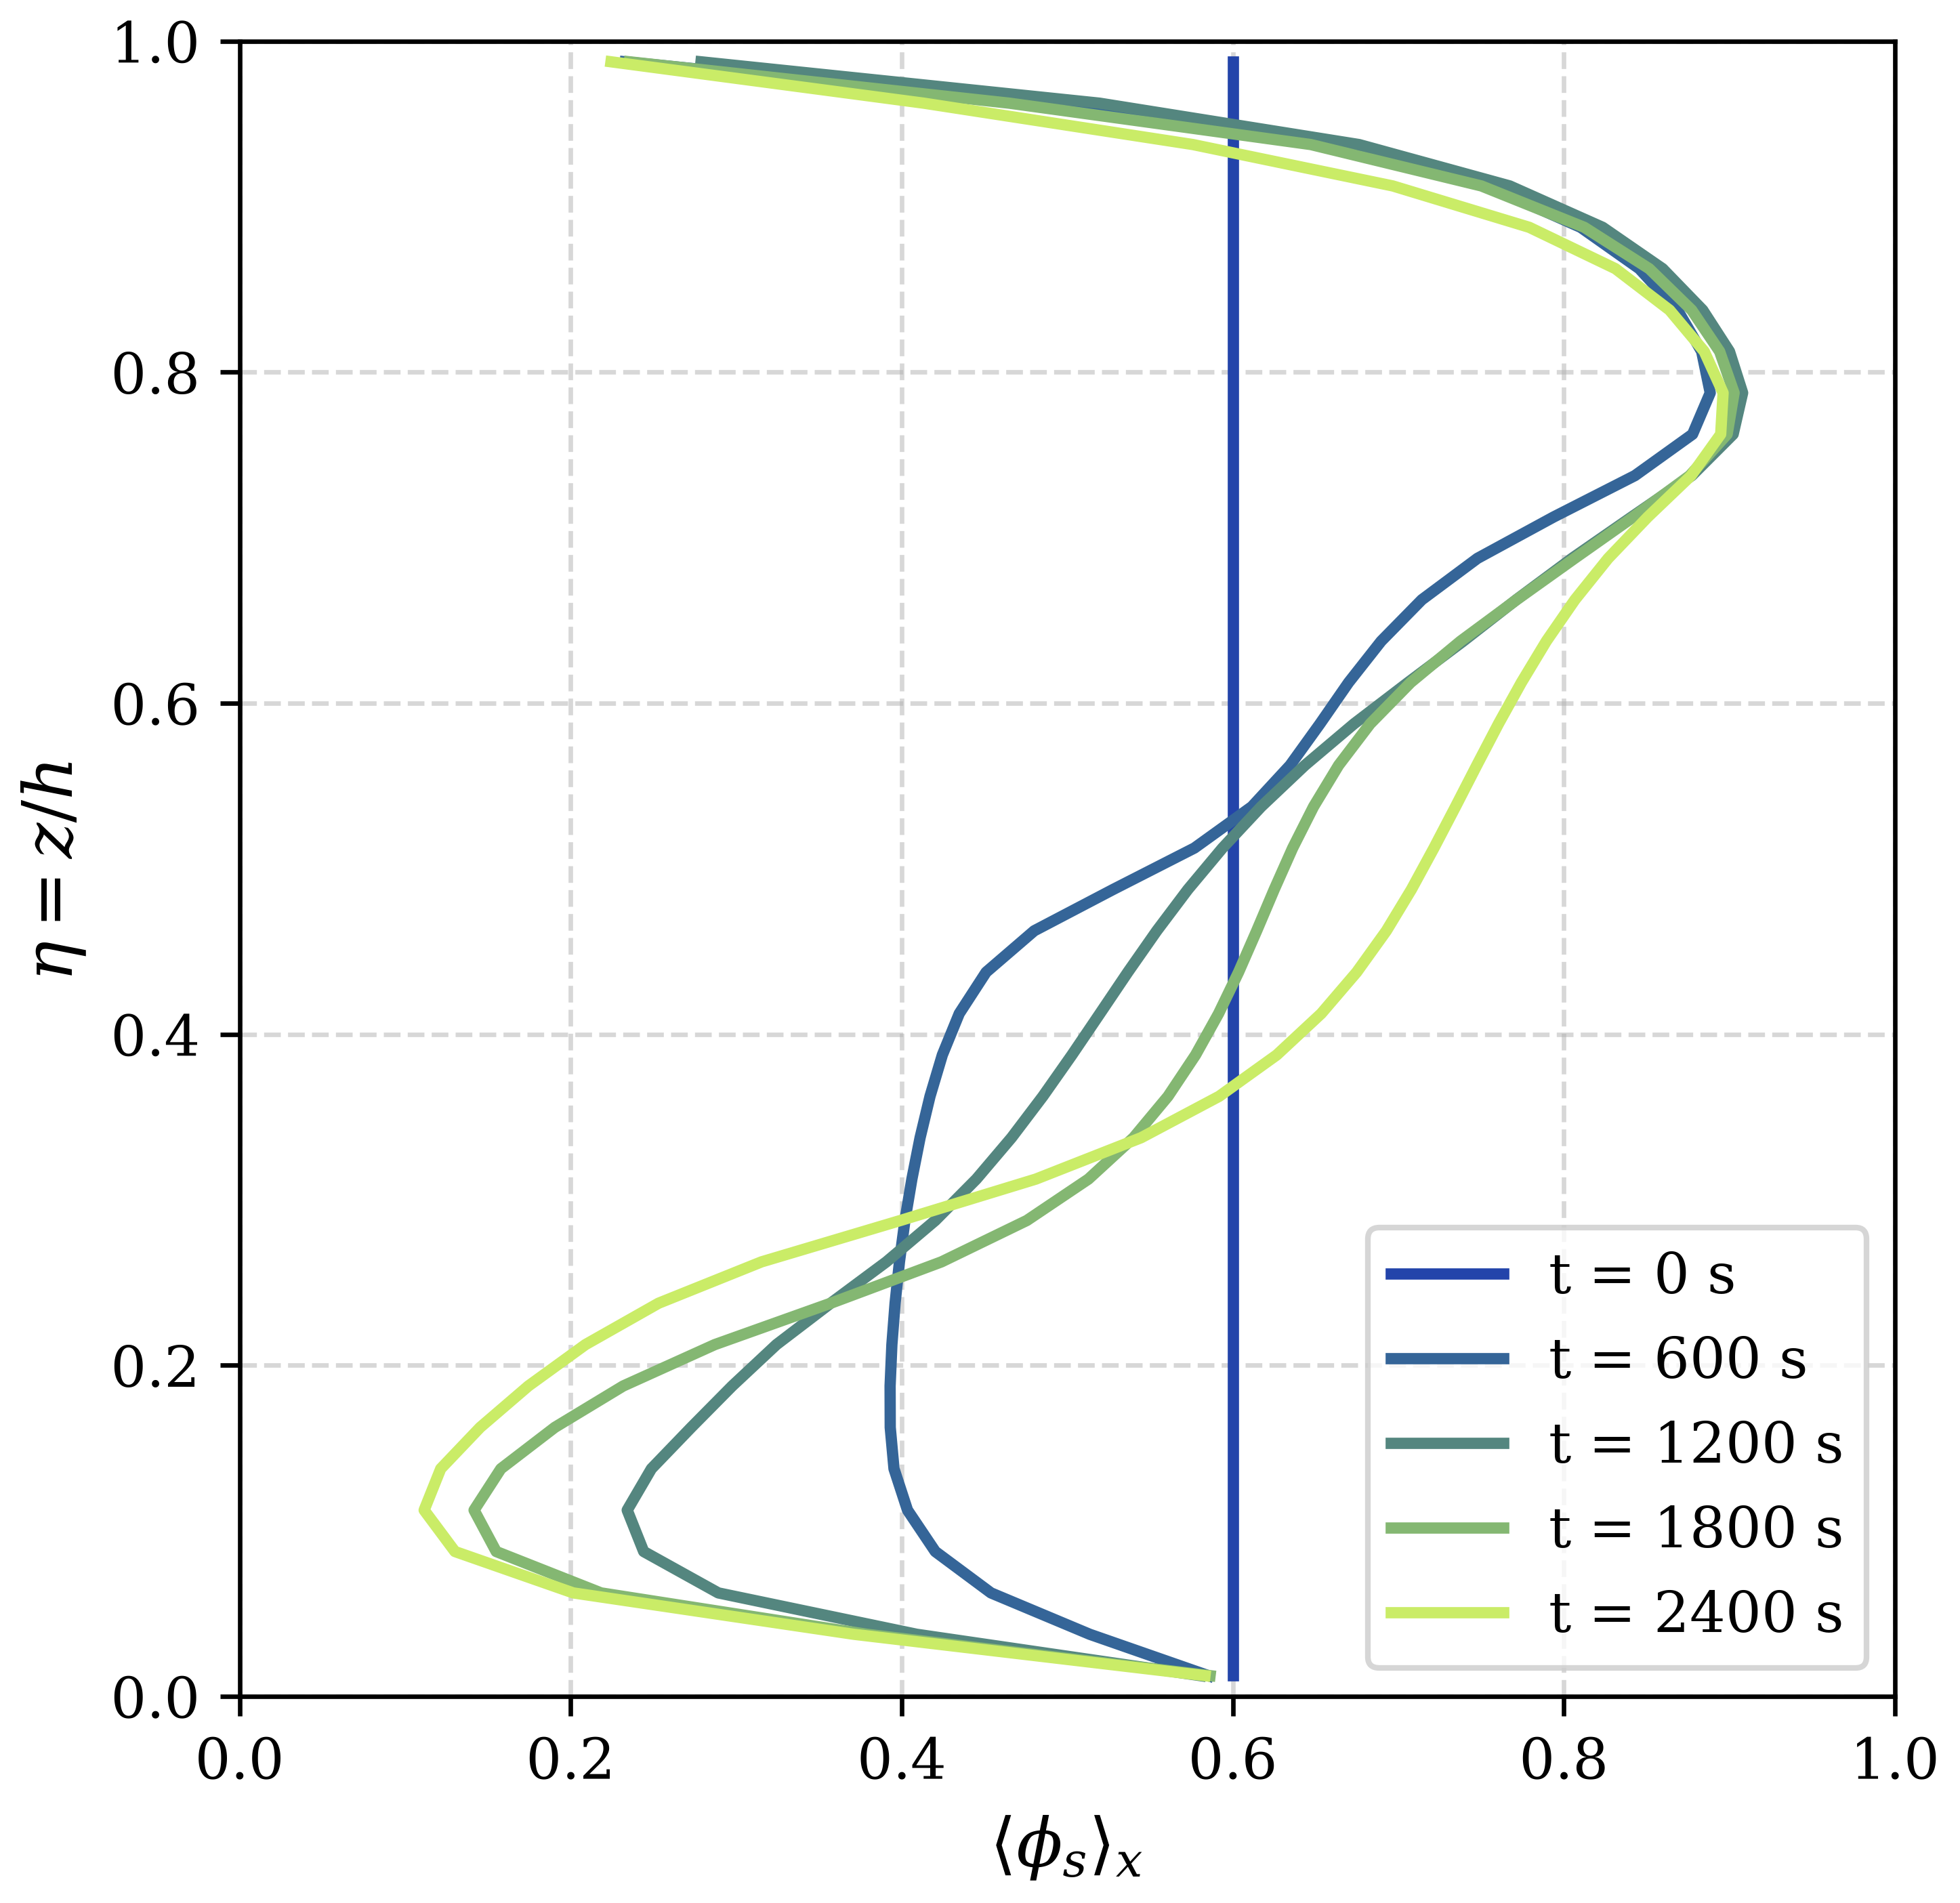
\includegraphics[width=\textwidth]{phi_s_vs_eta_time_phi60.png}
        \caption{Model}
    \end{subfigure}
    \caption{\textbf{Temporal evolution of the vertical sorting for $\phi_s^0 = 0.60$}. Left: Experimental data. Right: Model prediction.}
    \label{fig:phi60_time}
\end{figure}

\begin{figure}[H]
    \centering
    \begin{subfigure}[t]{0.48\textwidth}
        \centering
        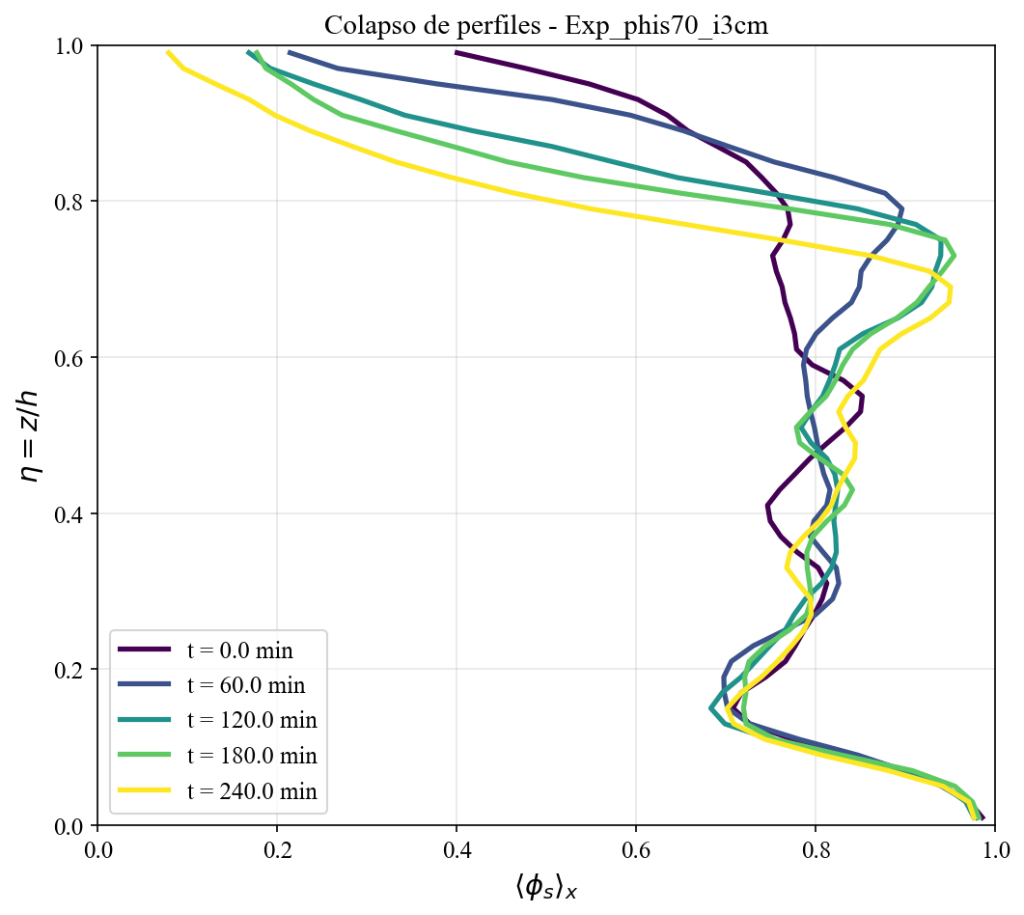
\includegraphics[width=\textwidth]{Exp_phis70_time.png}
        \caption{Experimental}
    \end{subfigure}
    \hfill
    \begin{subfigure}[t]{0.48\textwidth}
        \centering
        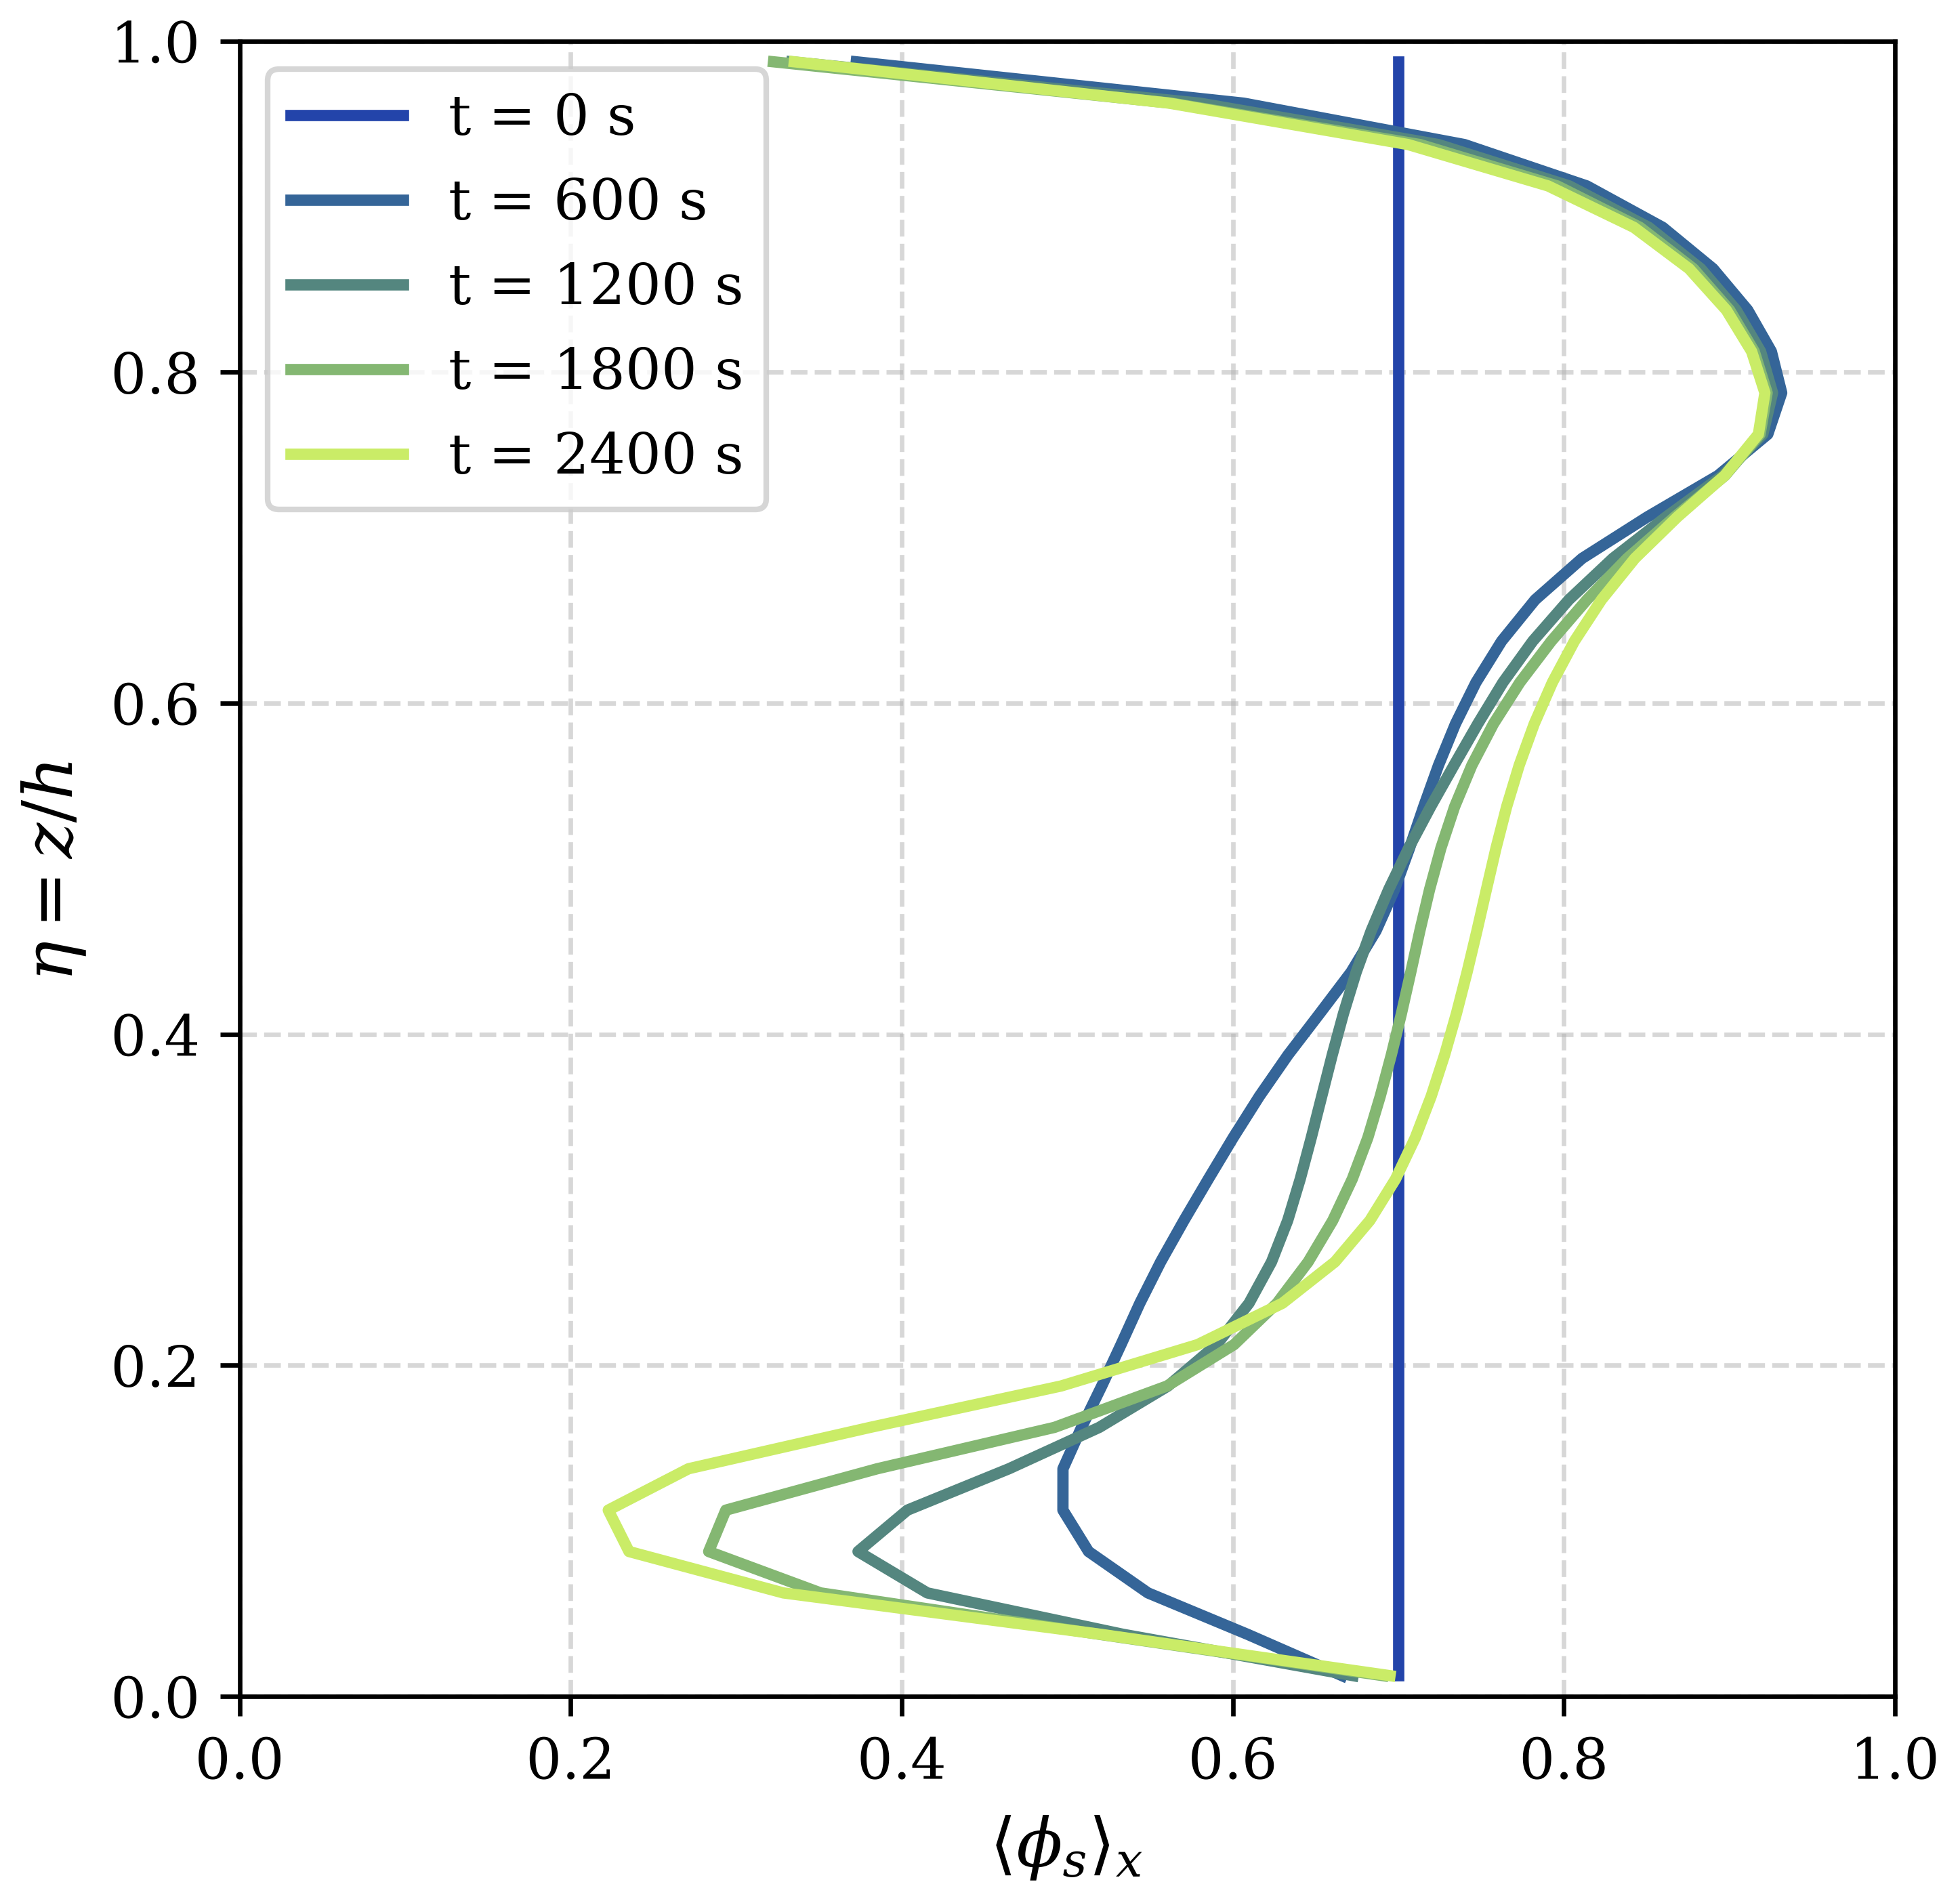
\includegraphics[width=\textwidth]{phi_s_vs_eta_time_phi70.png}
        \caption{Model}
    \end{subfigure}
    \caption{\textbf{Temporal evolution of the vertical sorting for $\phi_s^0 = 0.70$}. Left: Experimental data. Right: Model prediction.}
    \label{fig:phi70_time}
\end{figure}

\begin{figure}[H]
    \centering
    \begin{subfigure}[t]{0.48\textwidth}
        \centering
        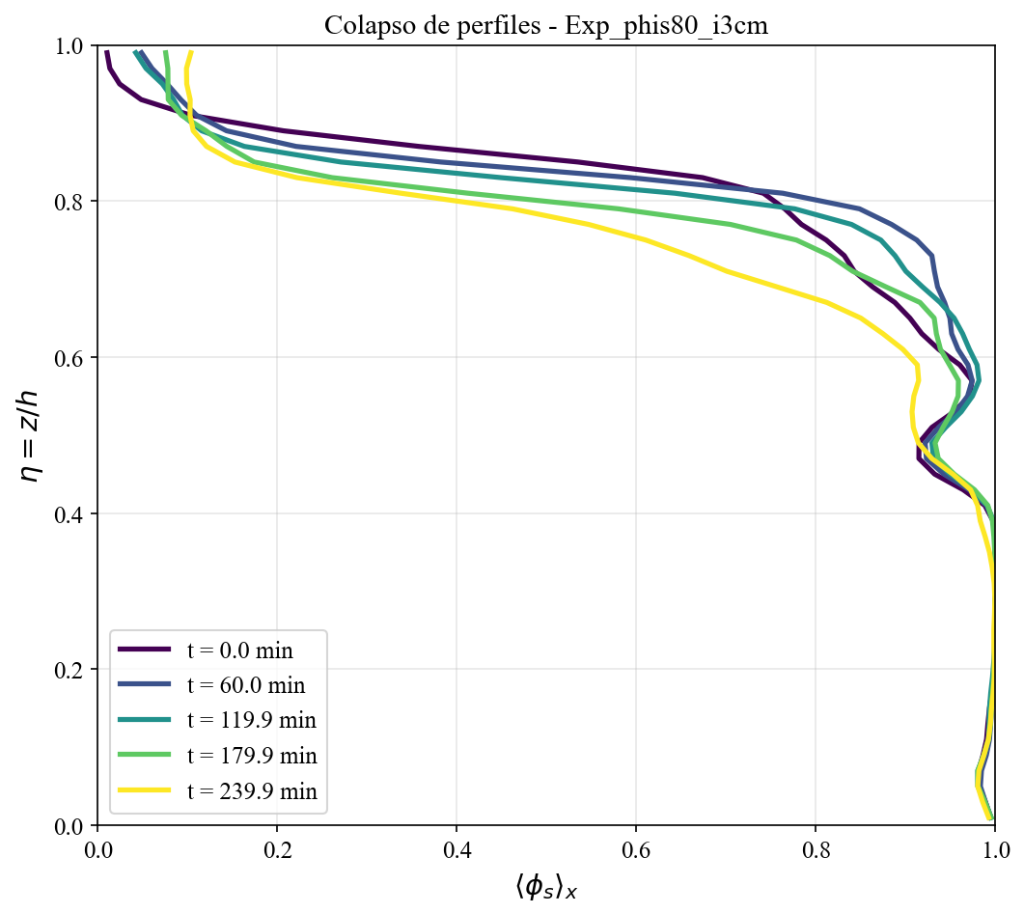
\includegraphics[width=\textwidth]{Exp_phis80_time.png}
        \caption{Experimental}
    \end{subfigure}
    \hfill
    \begin{subfigure}[t]{0.48\textwidth}
        \centering
        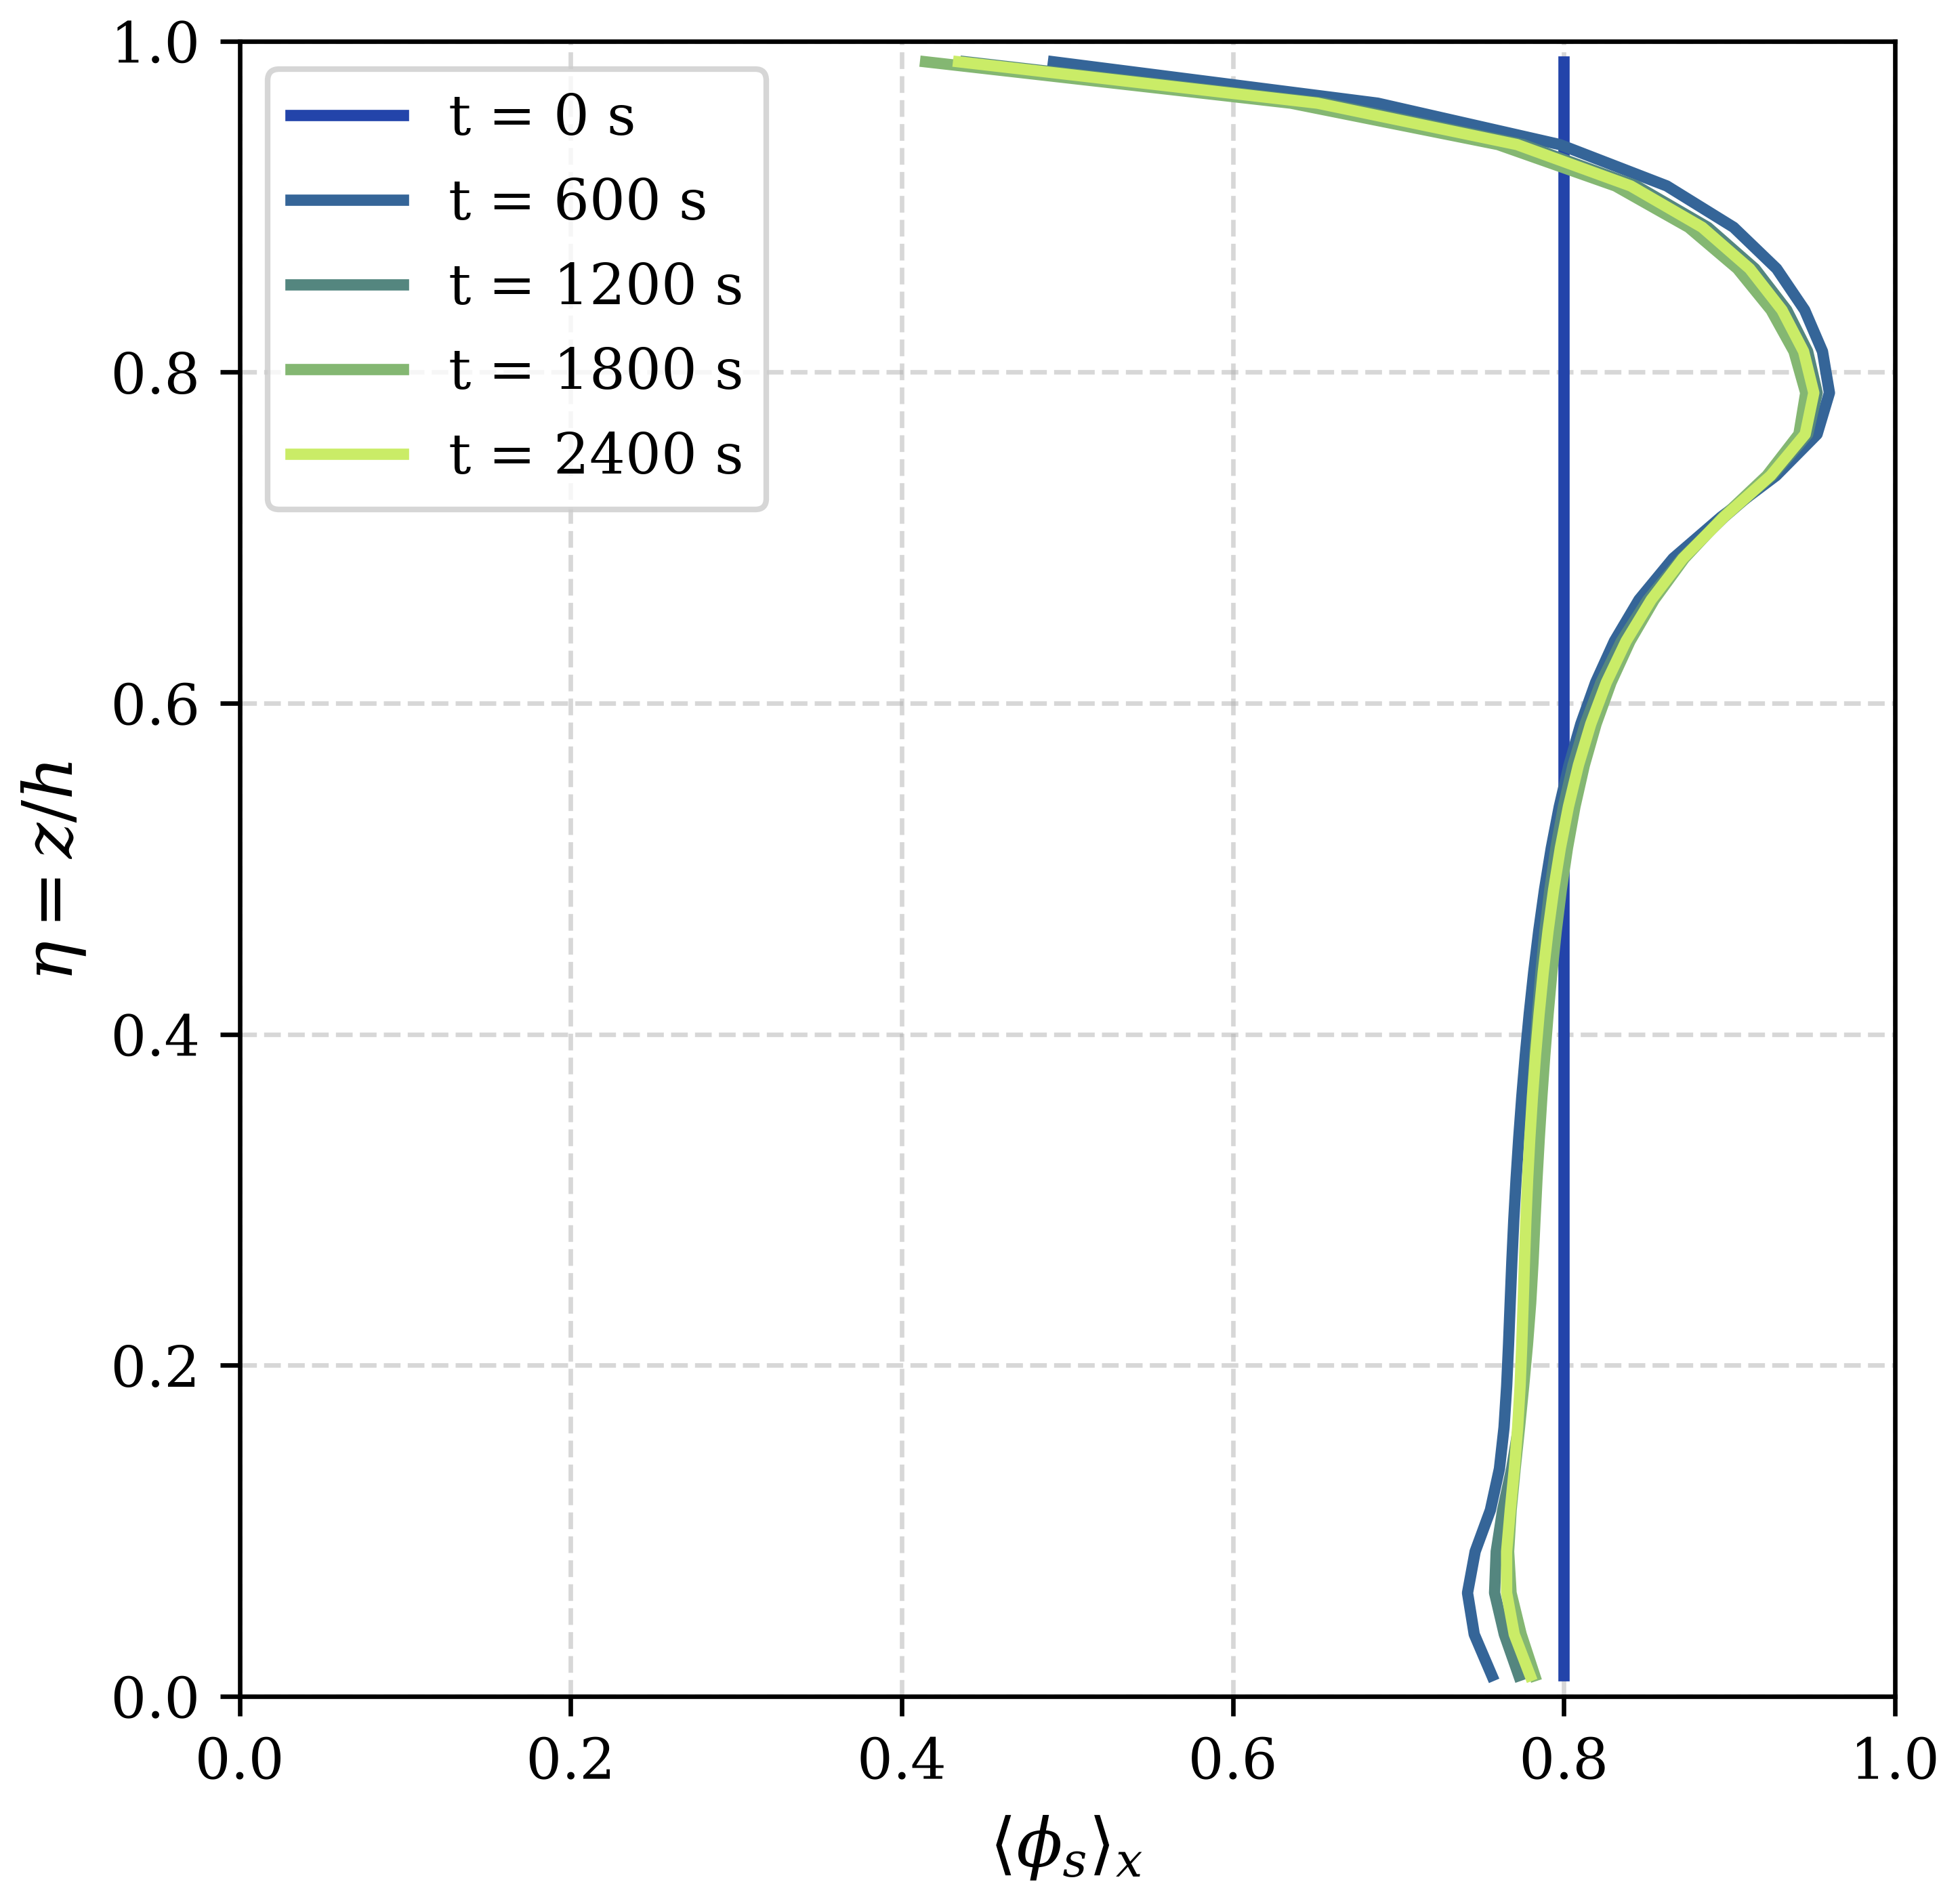
\includegraphics[width=\textwidth]{phi_s_vs_eta_time_phi80.png}
        \caption{Model}
    \end{subfigure}
    \caption{\textbf{Temporal evolution of the vertical sorting for $\phi_s^0 = 0.80$}. Left: Experimental data. Right: Model prediction.}
    \label{fig:phi80_time}
\end{figure}

\begin{figure}[H]
    \centering
    \begin{subfigure}[t]{0.48\textwidth}
        \centering
        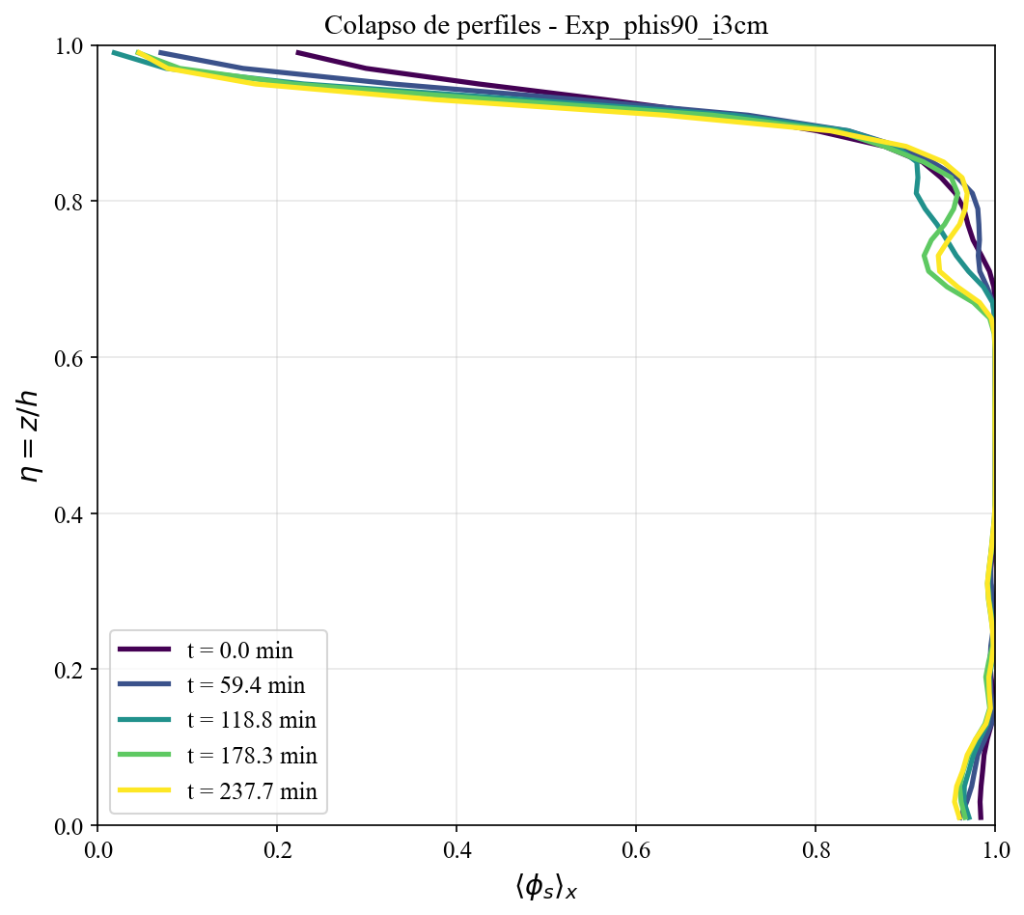
\includegraphics[width=\textwidth]{Exp_phis90_time.png}
        \caption{Experimental}
    \end{subfigure}
    \hfill
    \begin{subfigure}[t]{0.48\textwidth}
        \centering
        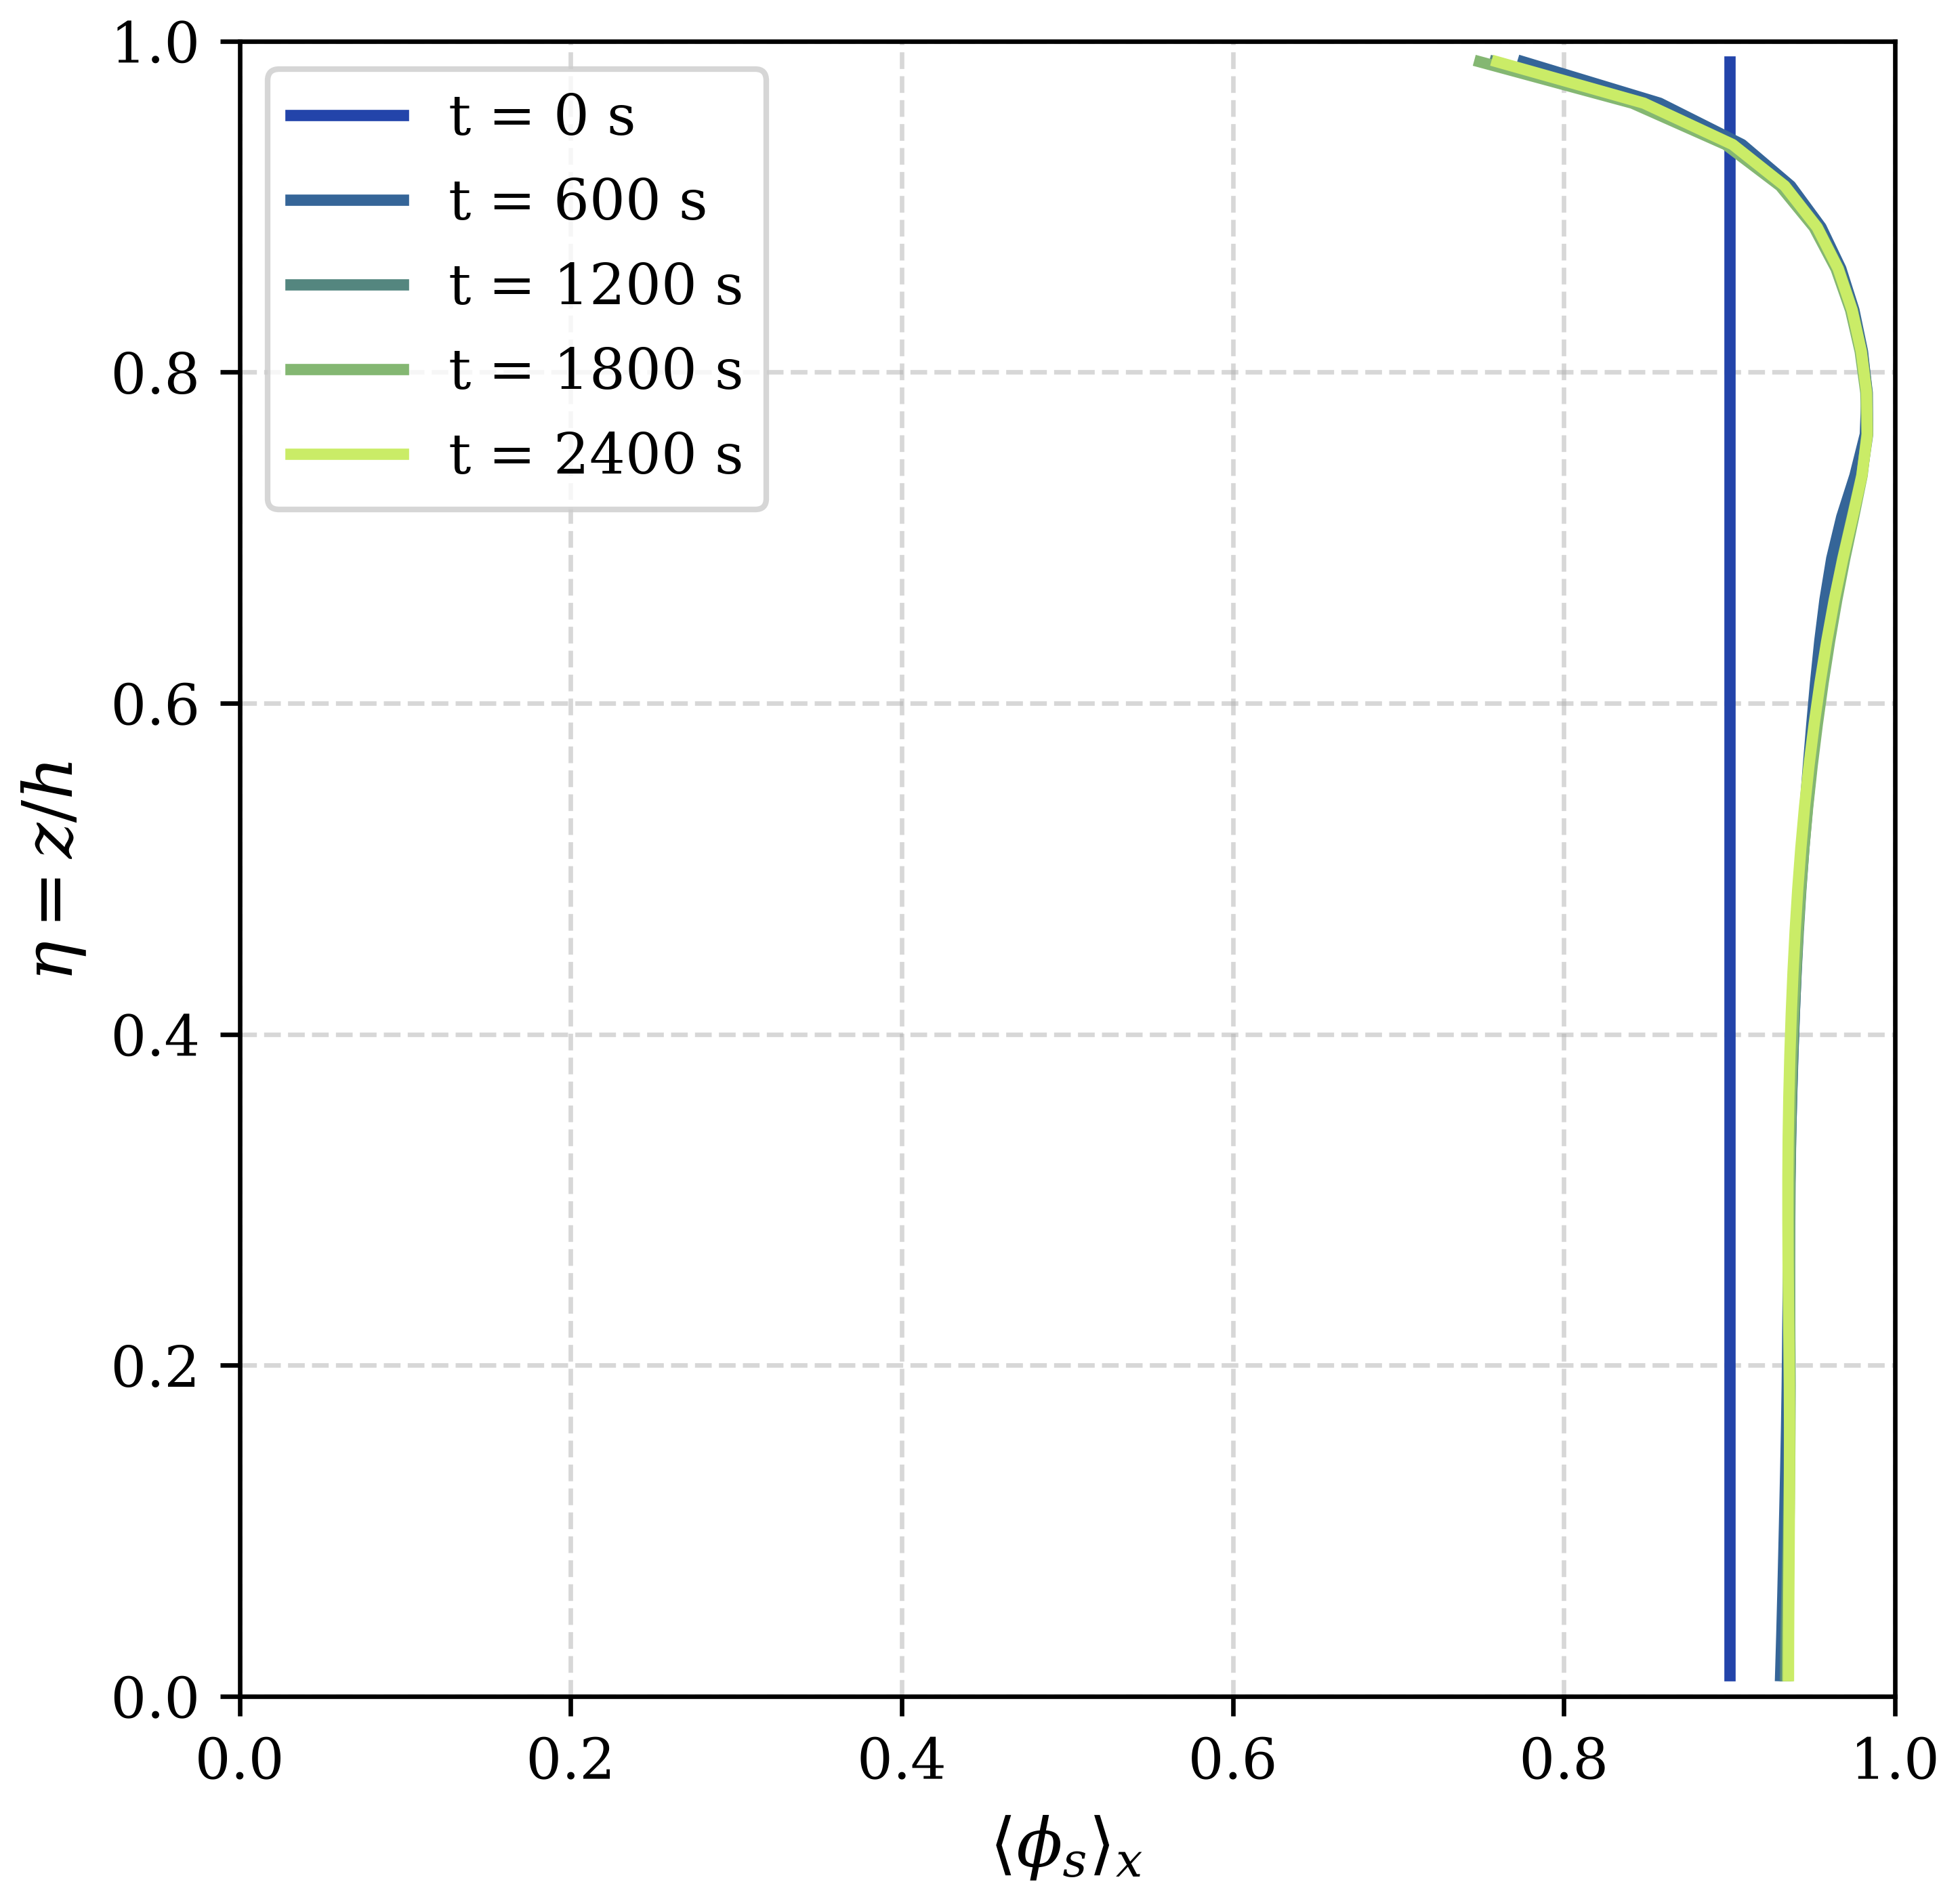
\includegraphics[width=\textwidth]{phi_s_vs_eta_time_phi90.png}
        \caption{Model}
    \end{subfigure}
    \caption{\textbf{Temporal evolution of the vertical sorting for $\phi_s^0 = 0.90$}. Left: Experimental data. Right: Model prediction.}
    \label{fig:phi90_time}
\end{figure}

\subsection*{Analysis and interpretation}

The side-by-side comparison of experimental data and model predictions across all initial concentrations reveals the \textbf{kinetics} of the segregation process. Both experimental and numerical profiles demonstrate three kinetic stages:

\begin{enumerate}
    \item \textit{Induction stage} ($t \lesssim 500$\,s): The profile is
          nearly unchanged from the initial uniform condition (dotted line).
          The velocity field is being established and the segregation flux
          has not yet had time to produce a visible effect on the column-averaged
          profile.
    \item \textit{Active transient} ($500 \lesssim t \lesssim 1800$\,s):
          The sorting front (Sec.~\ref{sec:diffusion}) descends rapidly.
          Fines accumulate in the middle layers of the column while coarse
          grains are expelled upward, building the characteristic three-layer
          structure.
    \item \textit{Deceleration} ($t \gtrsim 2000$\,s): The profile changes
          progressively slower as the system approaches the diffusive
          equilibrium within the active layer. The process does not fully
          stop within the simulation time (see Appendix~\ref{app:convergence}).
\end{enumerate}

The uniform initial condition (dotted line) serves as the reference for the
\emph{total change} from start to finish, which is the appropriate
denominator when normalizing convergence metrics.

\newpage
% ============================================================
\section{Equilibrium Length $\ell$ and Local Péclet Fields}
\label{sec:peclet}
% ============================================================

The heatmaps of $\ell$ and $Pe$ provide the quantitative framework that
explains \emph{why} the advective segregation flux dominates and what role
the lithostatic pressure plays in suppressing segregation at depth.

\begin{figure}[H]
    \centering
    \begin{subfigure}[b]{1.0\textwidth}
        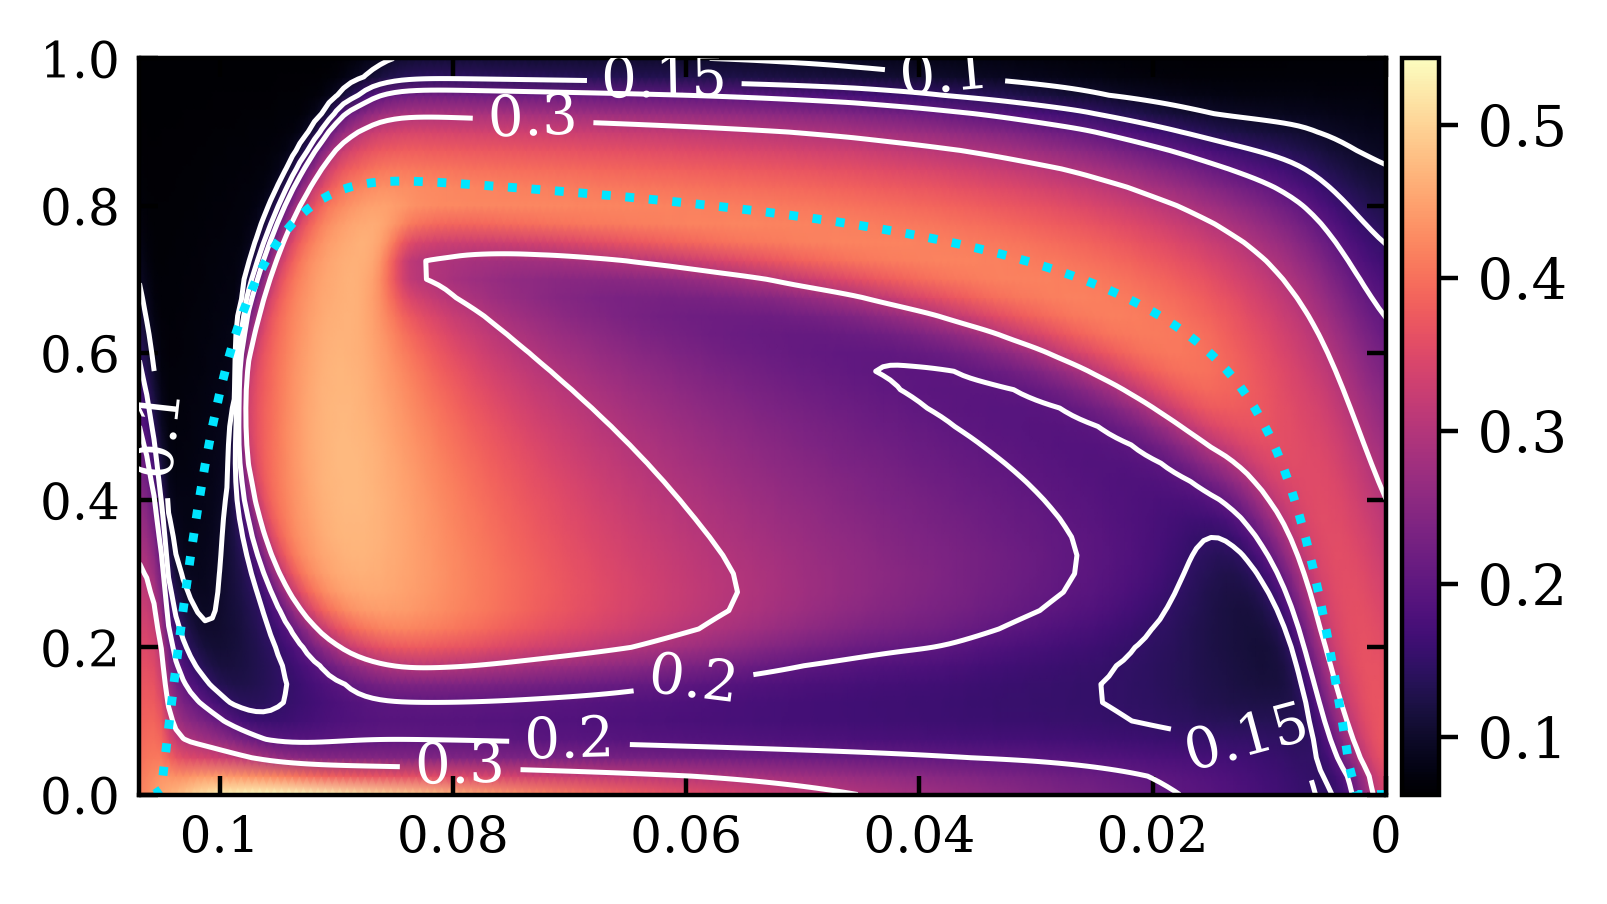
\includegraphics[width=\textwidth]{heatmap_l_individual.png}
    \end{subfigure}
    \vspace{0.3cm}
    
    \begin{subfigure}[b]{1.0\textwidth}
        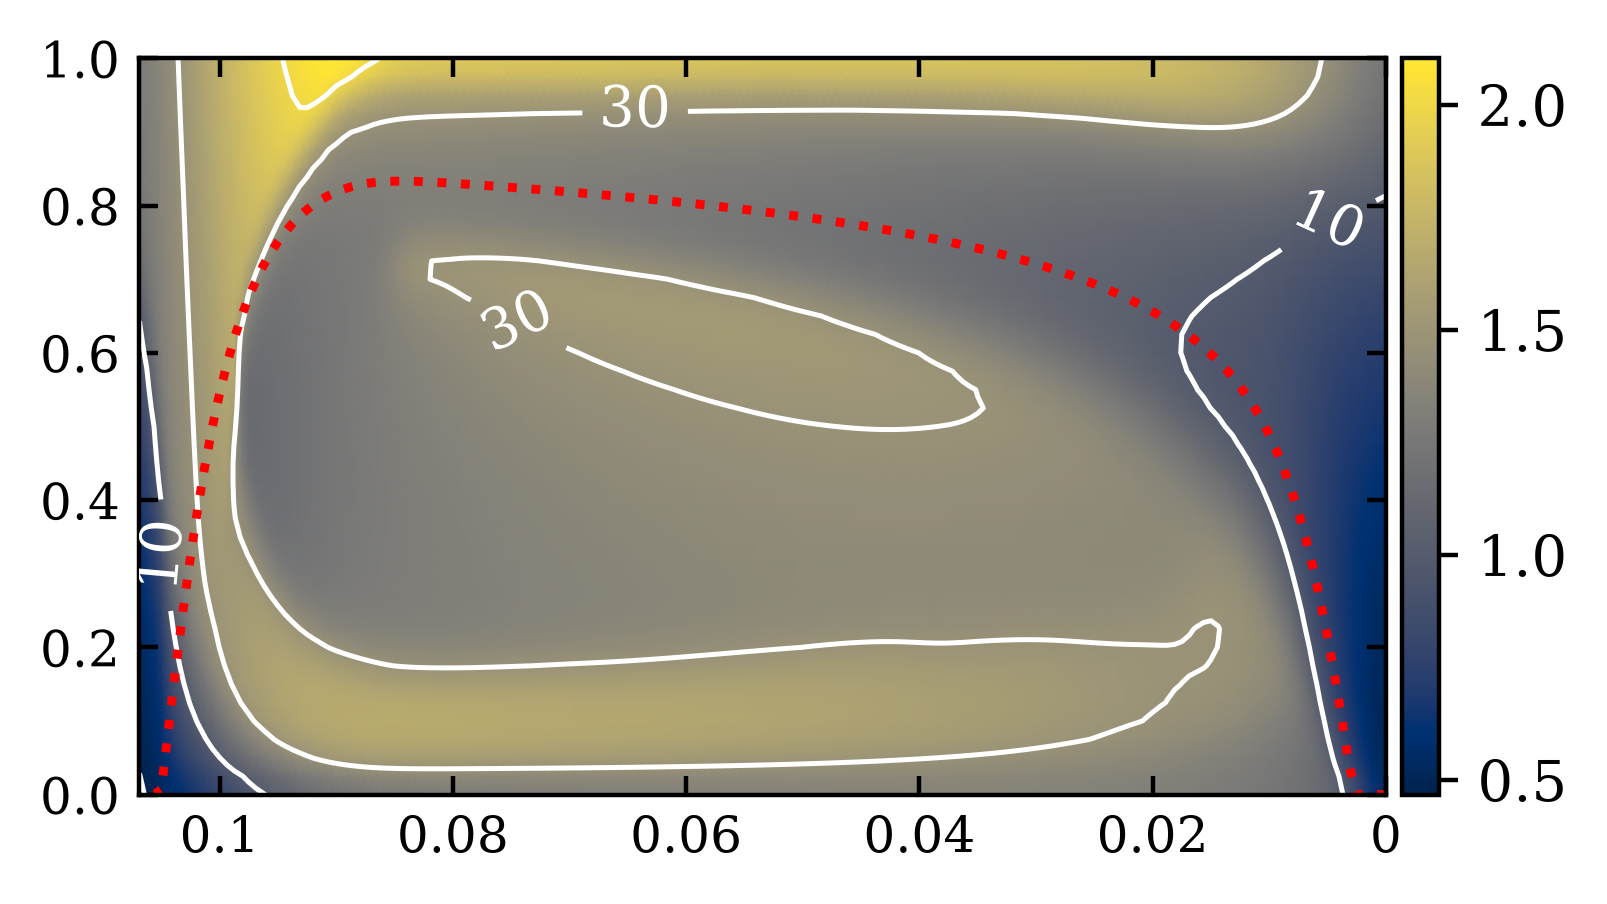
\includegraphics[width=\textwidth]{heatmap_Pe_individual.png}
    \end{subfigure}
    \caption{%
        \textbf{Spatial maps of $\ell(x,\eta)$ and $Pe(x,\eta)$} for
        $\phi_s^0 = 0.70$, with diffusion, $t = 2400$\,s.
        \textbf{Top}: map of the equilibrium length $\ell$ (mm) with
        white isolines. The increase of $\ell$ with depth reflects the
        growth of lithostatic pressure.
        \textbf{Bottom}: map of $\log_{10} Pe$ with white isolines.
        $Pe \gg 1$ throughout the dune confirms that segregation advection
        dominates over diffusion at all spatial locations.
    }
    \label{fig:heatmap70}
\end{figure}

\subsection*{Analysis and interpretation}

\paragraph{Map of $\ell$.}
The equilibrium length $\ell = D_{sl}/f_{sl}$ grows with depth because the
lithostatic pressure $p$ in the numerator of Eq.~(\ref{eq:ell}) increases
towards the base. Typical values range from
$\ell \approx 0.10$\,mm at the surface to $\ell \approx 0.30$\,mm at the
base (a factor of $\approx 8.7$). This implies that compositional interfaces
are inherently more diffuse at depth, independent of whether an explicit
diffusion term is included. The lithostatic pressure thus acts as a
\emph{natural depth-dependent regularization} of the hyperbolic problem.

\paragraph{Map of $Pe$.}
With $L = h$ (the full bed thickness as the reference length):
\begin{itemize}
    \item $Pe$ increases towards the surface (where pressure is low and
          $\ell$ is small) and towards the crest (where $h$ is largest).
    \item $Pe \gg 1$ throughout the entire dune: at the scale of the
          full column, \emph{segregation always dominates diffusion}.
\end{itemize}

Using the physically tighter scale $L = \delta_a$ (active layer
thickness) reduces $Pe$ considerably but does not invert the conclusion
at the reference station (lee 50\%, $h = 4.98$\,mm):

\begin{table}[H]
    \centering
    \begin{tabular}{lcc}
        \toprule
        & Surface & Base \\
        \midrule
        $Pe$ with $L = h$        & 79.8 & 9.2 \\
        $Pe$ with $L = \delta_a$ & 24.0 & 2.8 \\
        \bottomrule
    \end{tabular}
    \caption{Péclet number at the lee 50\% station.}
    \label{tab:Pe}
\end{table}

$Pe > 1$ everywhere in the column even with $L = \delta_a$, confirming
that segregation advection is dominant. The narrowest margin is at the
base ($Pe \approx 2.8$), where diffusion provides the strongest
relative broadening ---consistent with the wider interfaces seen at
depth in the $\ell$ map.

\paragraph{Note on the regularization floor.}
The comparison with and without $p_{\rm floor}$ shows that
$p_{\rm floor} \approx p_{\rm lit}^{\rm max}$: a fraction of the
depth-dependent suppression of segregation is numerical regularization
rather than genuine physical lithostatic pressure. This must be
declared explicitly in the paper.

\newpage
% ============================================================
\section{Summary of the Main Results}
% ============================================================

\begin{table}[H]
    \centering
    \renewcommand{\arraystretch}{1.4}
    \begin{tabular}{lp{10cm}}
        \toprule
        Figure & Main result \\
        \midrule
        Fig.~\ref{fig:fan} (§\ref{sec:fan}) &
            Global space--time picture. The sorting front propagates rapidly
            then slows; the pattern is spatially modulated by dune geometry
            and approaches (but does not reach) a traveling wave. \\
        Fig.~\ref{fig:F1} (§\ref{sec:sorting}) &
            Three universal compositional layers (coarse base, fines body,
            coarse surface crust). Diffusion reduces the gradation index by
            $\approx 20\%$. The index collapses for $\phi_s^0 \to 1$. \\
        Fig.~\ref{fig:F2} (§\ref{sec:velocity}) &
            The trapping of coarse grains is driven by a closed recirculation
            cell in the co-moving frame, \emph{not} by the kinematic
            stagnation point. Pearson anti-correlation $= -0.54$. \\
        Fig.~\ref{fig:comp_diffusion} (§\ref{sec:diffusion}) &
            Diffusion broadens interfaces and reduces contrasts by $\approx 20\%$
            but does not alter the topology of the recirculation cell or
            the three-layer structure. Interface thickness validated above
            the numerical mesh floor. \\
        Fig.~\ref{fig:diff_evol} (§\ref{sec:diffusion}) &
            The dynamic difference maps and zoom profiles reveal how the interface broadening induced by diffusion evolves and deepens continuously over time. \\
        Figs.~\ref{fig:phi50_time}--\ref{fig:phi90_time} (§\ref{sec:temporal}) &
            Three kinetic stages: induction, active transient, deceleration.
            The state at $t = 2400$\,s is representative but not fully
            converged (see Appendix~\ref{app:convergence}). \\
        Fig.~\ref{fig:heatmap70} (§\ref{sec:peclet}) &
            $Pe \gg 1$ throughout the dune with $L = h$; with $L = \delta_a$
            the margin narrows at the base. Lithostatic pressure naturally
            suppresses segregation in depth. \\
        Fig.~\ref{fig:estab} (App.~\ref{app:convergence}) &
            The system moves by $\sim 11.5\%$ of the total change between
            $t = 2400$ and $4800$\,s: not fully converged. \\
        \bottomrule
    \end{tabular}
    \caption{Synthesis of the key results by figure.}
    \label{tab:summary}
\end{table}

\subsection*{General conclusion}

The set of figures demonstrates that \textbf{bidisperse sedimentary segregation
in hydraulic dunes} produces a robust and repeatable compositional structure.
This structure is:

\begin{enumerate}
    \item \textbf{Qualitatively insensitive} to the hydraulic slope in the
          range $i \in [0.005, 0.014]$: the slope controls the speed of
          unmixing, not the sharpness of the interfaces ($\ell$ and $Pe$ do not
          depend on $i$ because $\dot{\gamma}$ cancels in $D_{sl}/f_{sl}$).
    \item \textbf{Quantitatively reduced} by granular diffusion by
          $\approx 20\%$, with no qualitative change in the trend.
    \item \textbf{Generated by advection}, not by kinematic stagnation: the
          trapping mechanism is closed recirculation in the co-moving frame
          (Thornton \& Gray 2008), with an anti-correlation
          $r = -0.54$ with respect to the position of $u = 0$.
    \item \textbf{Not completely steady} at $t = 2400$\,s: the field
          continues to evolve, although most of the transient has elapsed.
\end{enumerate}

\newpage
% ============================================================
\appendix
\section{Temporal Convergence Analysis}
\label{app:convergence}
% ============================================================

This appendix documents the degree to which the simulations have converged
at the reporting time $t = 2400$\,s. The analysis uses an extended run at
$t = 4800$\,s as a reference.

\begin{figure}[H]
    \centering
    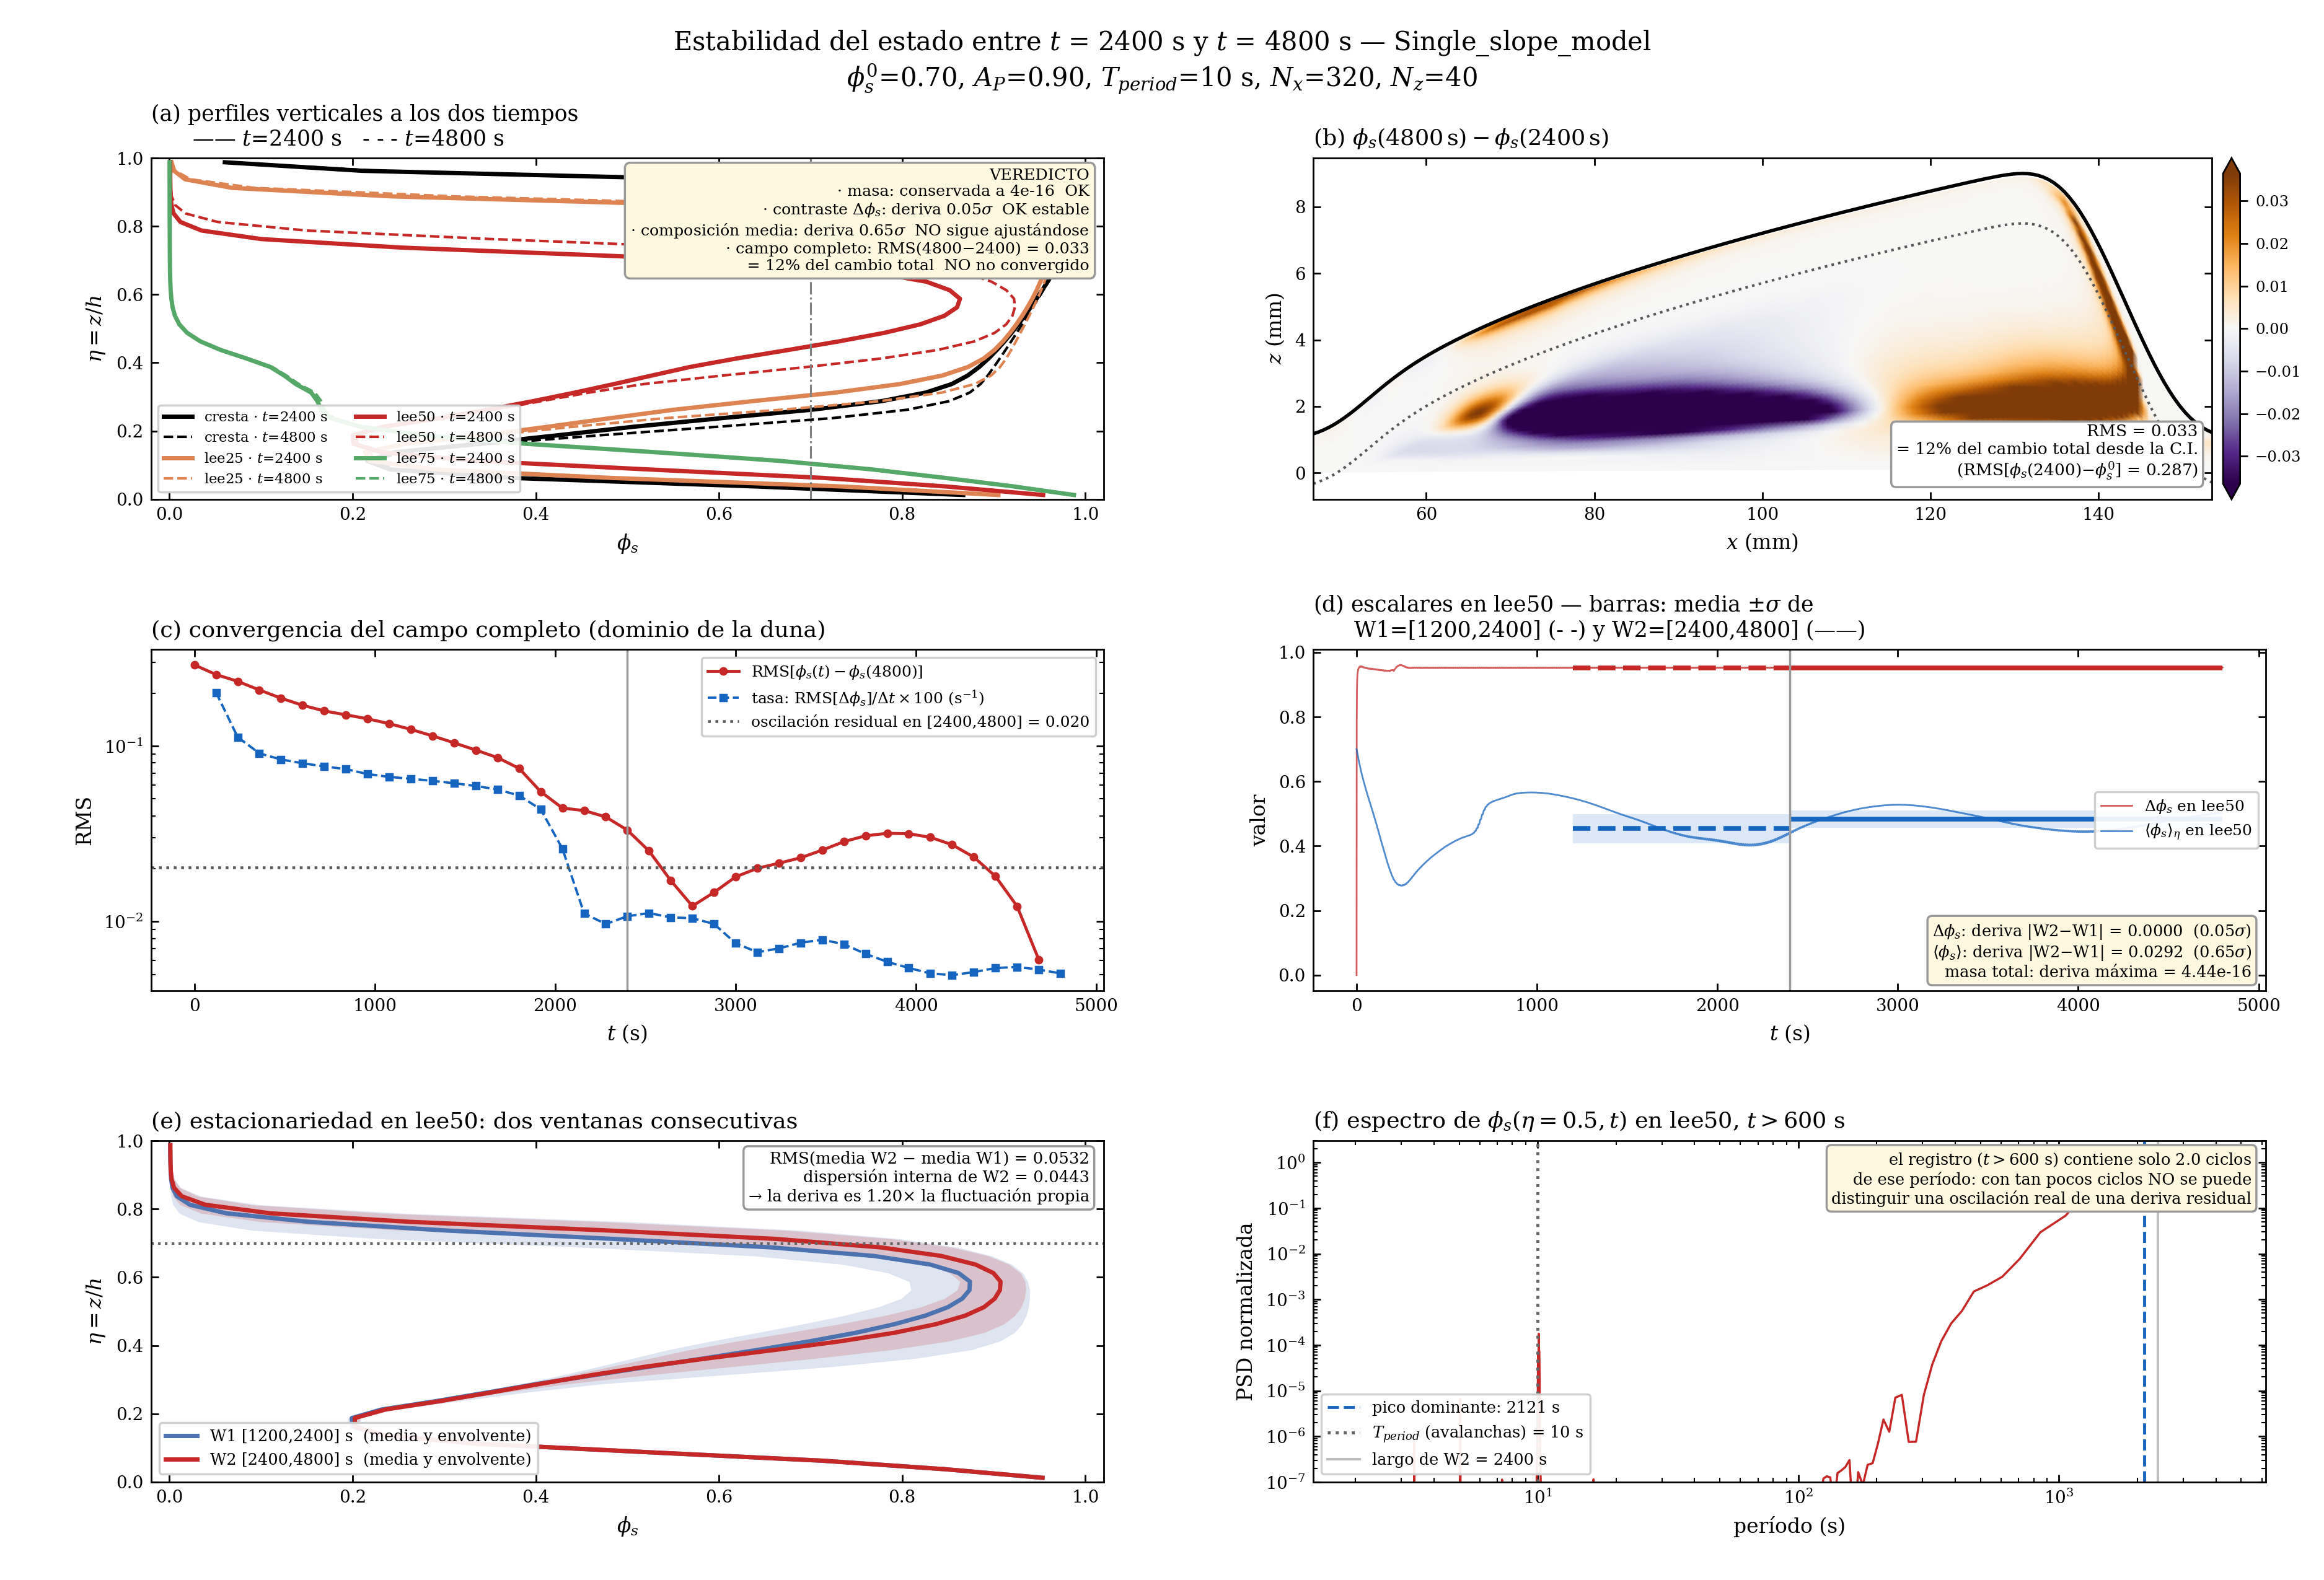
\includegraphics[width=\textwidth]{estabilidad_2400_4800.png}
    \caption{%
        \textbf{Temporal stability analysis}: comparison of the compositional
        field between $t = 2400$\,s and $t = 4800$\,s.
        The only extended run uses the \textit{Single slope model},
        mesh $N_x = 320$, $\phi_s^0 = 0.70$, with diffusion.
        The main panel shows the relative L$_2$ norm of the time-doubling
        test; the secondary panels show alternative metrics (geometric
        tracking of the coarse core and instantaneous rate of change).
    }
    \label{fig:estab}
\end{figure}

\subsection*{Time-doubling test}

For each instant $t$, the field is compared against its doubled time:
\[
    \epsilon(t) = \frac{\|\phi_s(t) - \phi_s(2t)\|_2}{\|\phi_s(2t)\|_2}
\]

\begin{table}[H]
    \centering
    \begin{tabular}{lc}
        \toprule
        Magnitude & Value \\
        \midrule
        Relative L$_2$ norm at $t = 2400$\,s & 0.046 \\
        Minimum value (at $t \approx 2040$\,s) & 0.025 \\
        $\|\phi(4800) - \phi(0)\|$ (total change) & 23.16 \\
        $\|\phi(2400) - \phi(4800)\|$ & 2.65 \\
        Fraction of total change between 2400 and 4800\,s & $\approx 11.5\%$ \\
        \bottomrule
    \end{tabular}
    \caption{Convergence metrics of the run extended to 4800\,s.}
    \label{tab:estab}
\end{table}

\paragraph{Correct interpretation.}
The denominator $\|\phi_s(2t)\|_2$ is dominated by the mean composition
($\langle\phi_s\rangle \approx 0.667$), not by the structural variation.
When the residual is instead normalized by the \emph{total change from
the initial condition}, the system is found to have moved
$\sim 11.5\%$ between $t = 2400$ and $4800$\,s. The state at $t = 2400$\,s
is therefore representative of the late-transient regime but is not an
equilibrium: reporting it as ``steady'' requires an explicit caveat.

\paragraph{Alternative metrics.}
The geometric tracking of the coarse core (mean $\eta$ position of the
$\phi_s$ minimum below $\eta_a$) confirms that the core continues to
descend slowly beyond $t = 2400$\,s. The instantaneous rate of change
$d\|\phi_s\|/dt$ decays monotonically after $t \approx 2040$\,s,
confirming that the system is decelerating but not halting within the
simulated window.

\end{document}
